\chapter{Application to fluvial flooding and analysis of the impacts of grid resolution and parameterisation}
\label{chapter:Fluvial}

The previous chapter considered a wide range of cases to evaluate the software's numerical and computational performance. It is necessary to simulate flooding at the scale of entire cities, to reproduce recent events such as the flooding in Carlisle (2005), New Orleans (2005), Hull (2007), Morpeth (2008), Leeds (2015), and Whitby (2016). Simulation of these complex urban environments requires advances in software, as described previously, to deliver results in a timely manner. This becomes even more pertinent for applications in real-time flood simulation, for incident management and forecasting. In doing so, new problems are also presented, such as the transferability of parameterisations between different grid resolutions, and the resolution beyond which diminishing returns are expected.

This chapter considers these practical matters of parameterisation and transferability, starting by applying the high-performance computing methods to simulate a real-world fluvial flood event, caused by defence overtopping, and comparing the results with a range of grid resolutions and parameters, to one of the most comprehensive post-event survey datasets available. A defence failure event is then considered, which in the absence of a suitable real-world dataset, is simulated as a hypothetical event near London used elsewhere in literature, with relative comparisons.

\section{Flooding in Carlisle, January 2005}

The new software has been applied to simulate flooding in Carlisle, North West England, in January 2005. Over 200mm of rain fell in a few hours over the Cumbrian mountains, believed to be equivalent to a \(1\%\) annual exceedance probability (AEP) event. Rivers quickly responded, with a volumetric discharge exceeding 1,500 m\textsuperscript{3}s\textsuperscript{-1} recorded within Carlisle itself on the River Eden, downstream of its major tributaries, the Rivers Petteril and Caldew. Severe flooding ensued, in an event that played out over more than 48 hours, affecting over 6,000 residents and directly flooding over 1,900 properties \citep{GONW2005,EnvironmentAgency2006a}.

In the week that followed both the Environment Agency (EA) and Bristol University conducted differential global positioning system (DGPS) surveys of water and wrack marks, their combined efforts creating one of the most comprehensive validation datasets for modelling urban flood inundation with 263 individual points. Different software codes and modelling techniques have since been applied to reproduce the event, most notably \citet{Neal2009}, \citet{Horritt2010}, \citet{Fewtrell2011a} and \citet{Liu2013}.

\begin{figure*}[tpb]
\centering
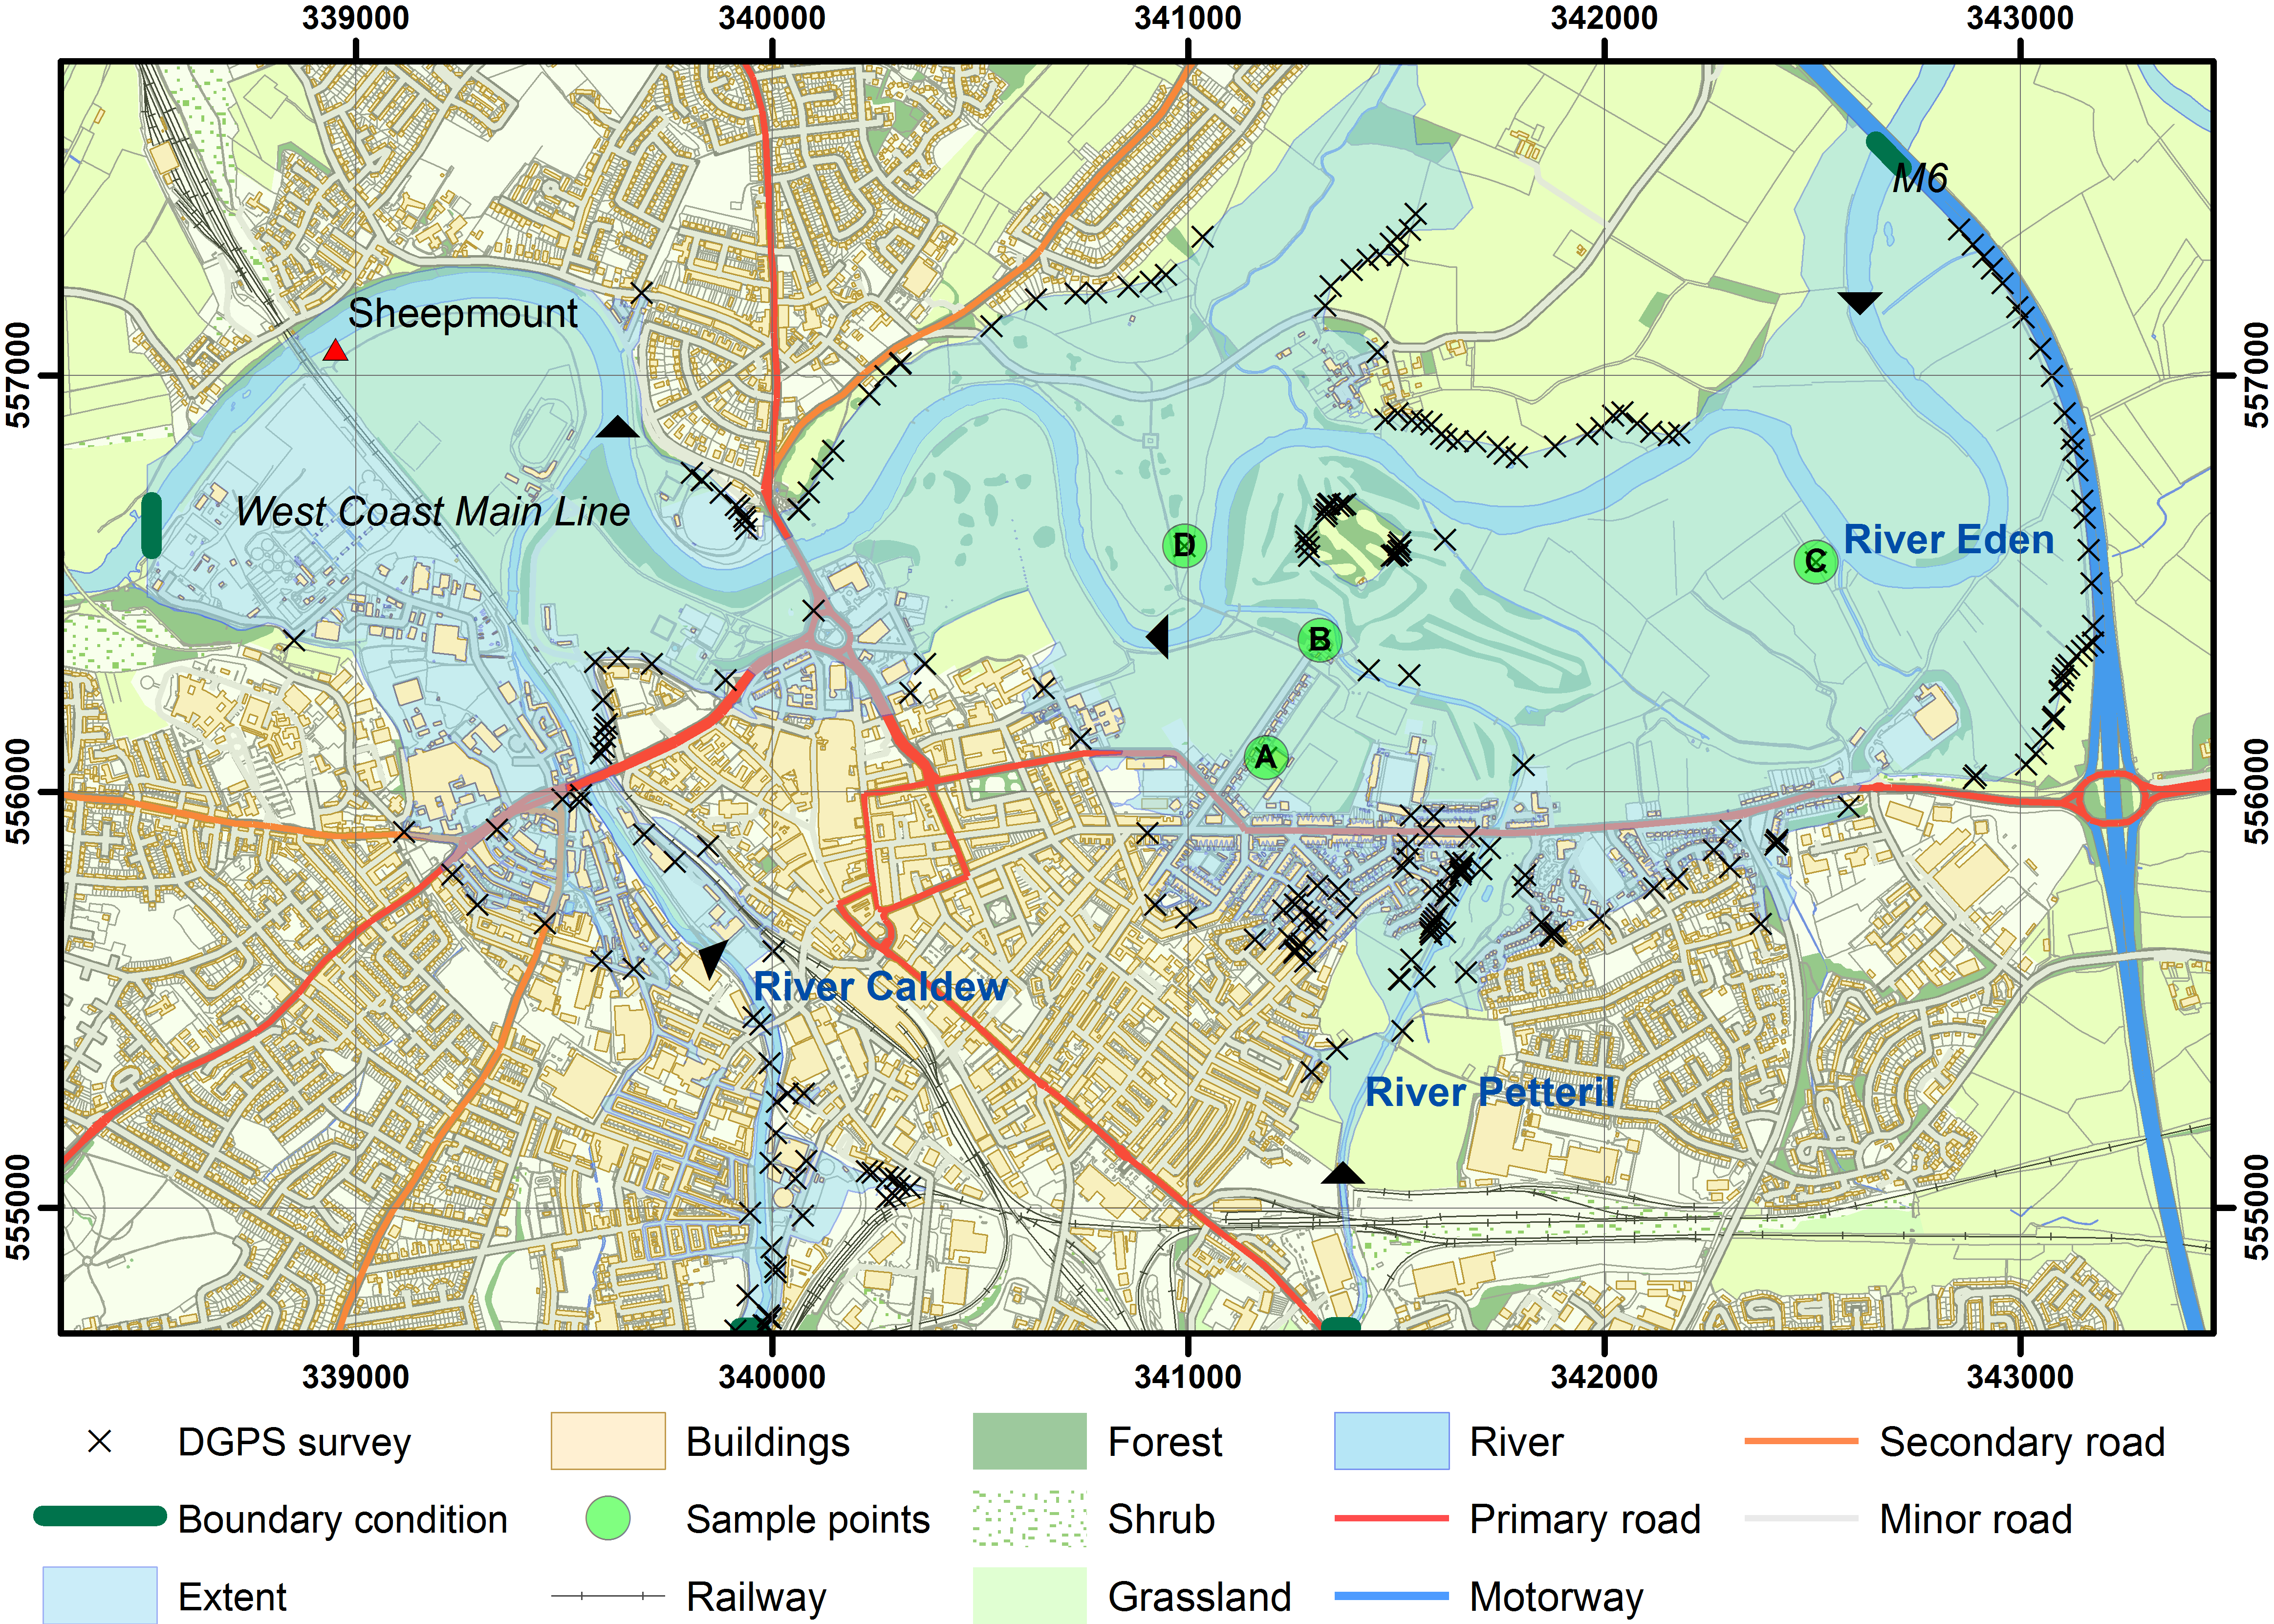
\includegraphics[width=1.0\textwidth]{carlisle-figures/Figure3.png}
\caption{Extent and topographic features for Carlisle with the three rivers and flow directions indicated.}
\floatfoot{Topographic data used in figure is \copyright{} Crown Copyright/database right 2013. An Ordnance Survey/EDINA supplied service.}
\label{CarlisleMap}
\end{figure*}
\begin{figure*}[tpb]
\centering
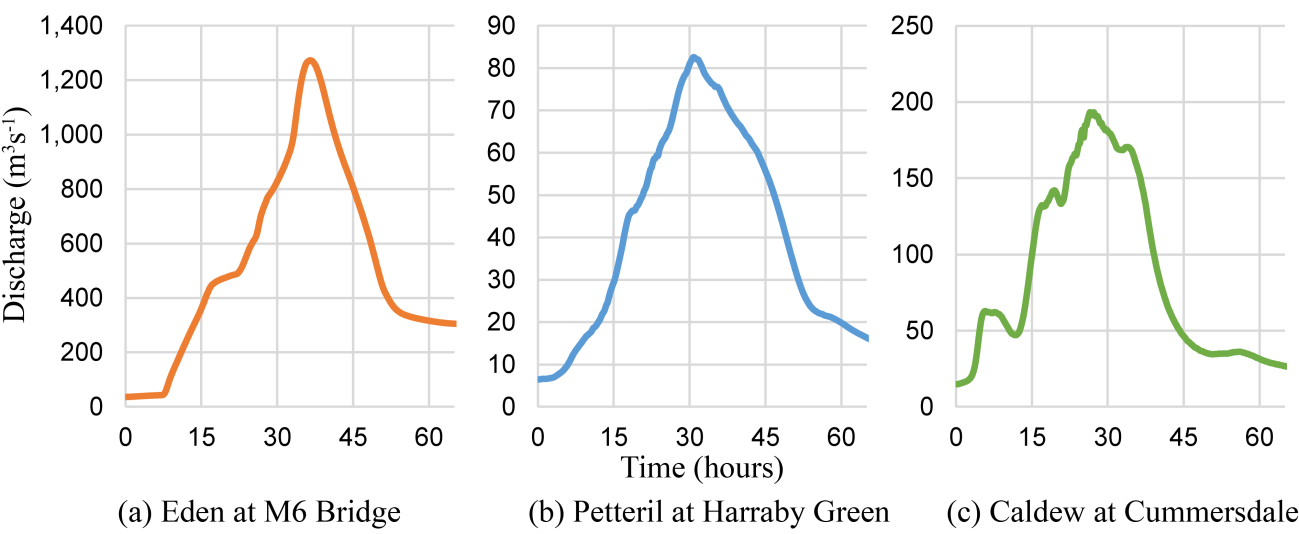
\includegraphics[width=0.9\textwidth]{carlisle-figures/Figure4.png}
\caption{Volumetric discharge inflow for the three rivers during the event.}
\label{BoundaryDischarges}
\end{figure*}

The topographic features, three rivers concerned, location of validation points, and approximate extent of the flood are shown in Figure \ref{CarlisleMap}. The root mean square error (RMSE) of the DGPS measurements is believed to be approximately 0.5m. The extent is deduced from a combination of EA records and the survey points, hence has buildings removed to create an appropriate mask for use with a high-resolution digital elevation model (DEM); for clarity this is different to the extent used by \citet{Horritt2010}. Inflow hydrographs for the three rivers are shown in Figure \ref{BoundaryDischarges}. The effects of rainfall within the city are neglected herein, to allow comparison with other published studies reproducing the event, and also because data is lacking for the sewer network and there is only anecdotal evidence detailing the sewer surcharging. 

\subsection{Model generation}

Fluvial flooding, in which defences are over-topped typically results in both slow velocities and a gradual evolution of the flood extent, except in cases where the defences are substantially overwhelmed, or fail completely. The nature of a gradual flood inundation event is such that minimal shocks would be expected, thus a first-order solution is considered to be an appropriate choice.

The topography for the model is produced from 2m DTM data provided by the Environment Agency Geomatics Group (EAGG). This product represents the lowest return value from the altimetric LiDAR surveys conducted, with interpolation (typically on a TIN basis) used to address any gaps. This generally provides a high quality representation of the ground level except in densely forested areas, in the author's experience. The highest return values represent the DEM product (referred to as DSM by EAGG), and include buildings but also street furniture, trees and shrubs. These latter items all create a partial barrier to flow, but not an absolute barrier. To ensure only buildings are included from the DEM, an extract is clipped using building outlines from Ordnance Survey's MasterMap product, and superimposed on the DTM data. No consideration is given herein to the partial obstructions created by street furniture, trees and shrubs, but it is recognised that some authors use sub-grid parameterisation or increase the roughness coefficient to address this \citep[e.g.][]{Bates2003,Yu2006,Casas2010,Chen2012}.

The LiDAR data obtained by EAGG cannot penetrate water to a substantial depth, thus is inadequate for representing the main channel of rivers. Data from a cross-sectional survey was interpolated along a spline of the river centreline to create a gradually-transitioning representation of the river bed, referenced against the same datum as the LiDAR data. This was superimposed atop the aforementioned DEM/DTM blend data, thereby excluding buildings which cantilever over the river, and with bridge supports manually added back to the data afterwards, perchance they should create a noteworthy flow constriction and backwater effect.

Once calibrated, simulations were executed with three different processing devices from each of the mainstream vendors to compare run-times. CPU simulations at high resolutions even using all four cores of the Intel Xeon E5-2609 would have taken several days to complete, hence were not run to completion. The vendor-quoted computational power of the two devices is 77 GFLOPS for the Intel Xeon E5-2609 \citep{IntelCorporation2012}, and 515 for the NVIDIA Tesla M2075 \citep{NVIDIACorporation2011}, representing a theoretical improvement of 6.7 times for the scientific GPU. The calibration procedure is described in the next section.

\subsection{Effect of grid resolution and parameterisation}

\begin{figure*}[tpb]
	\centering
	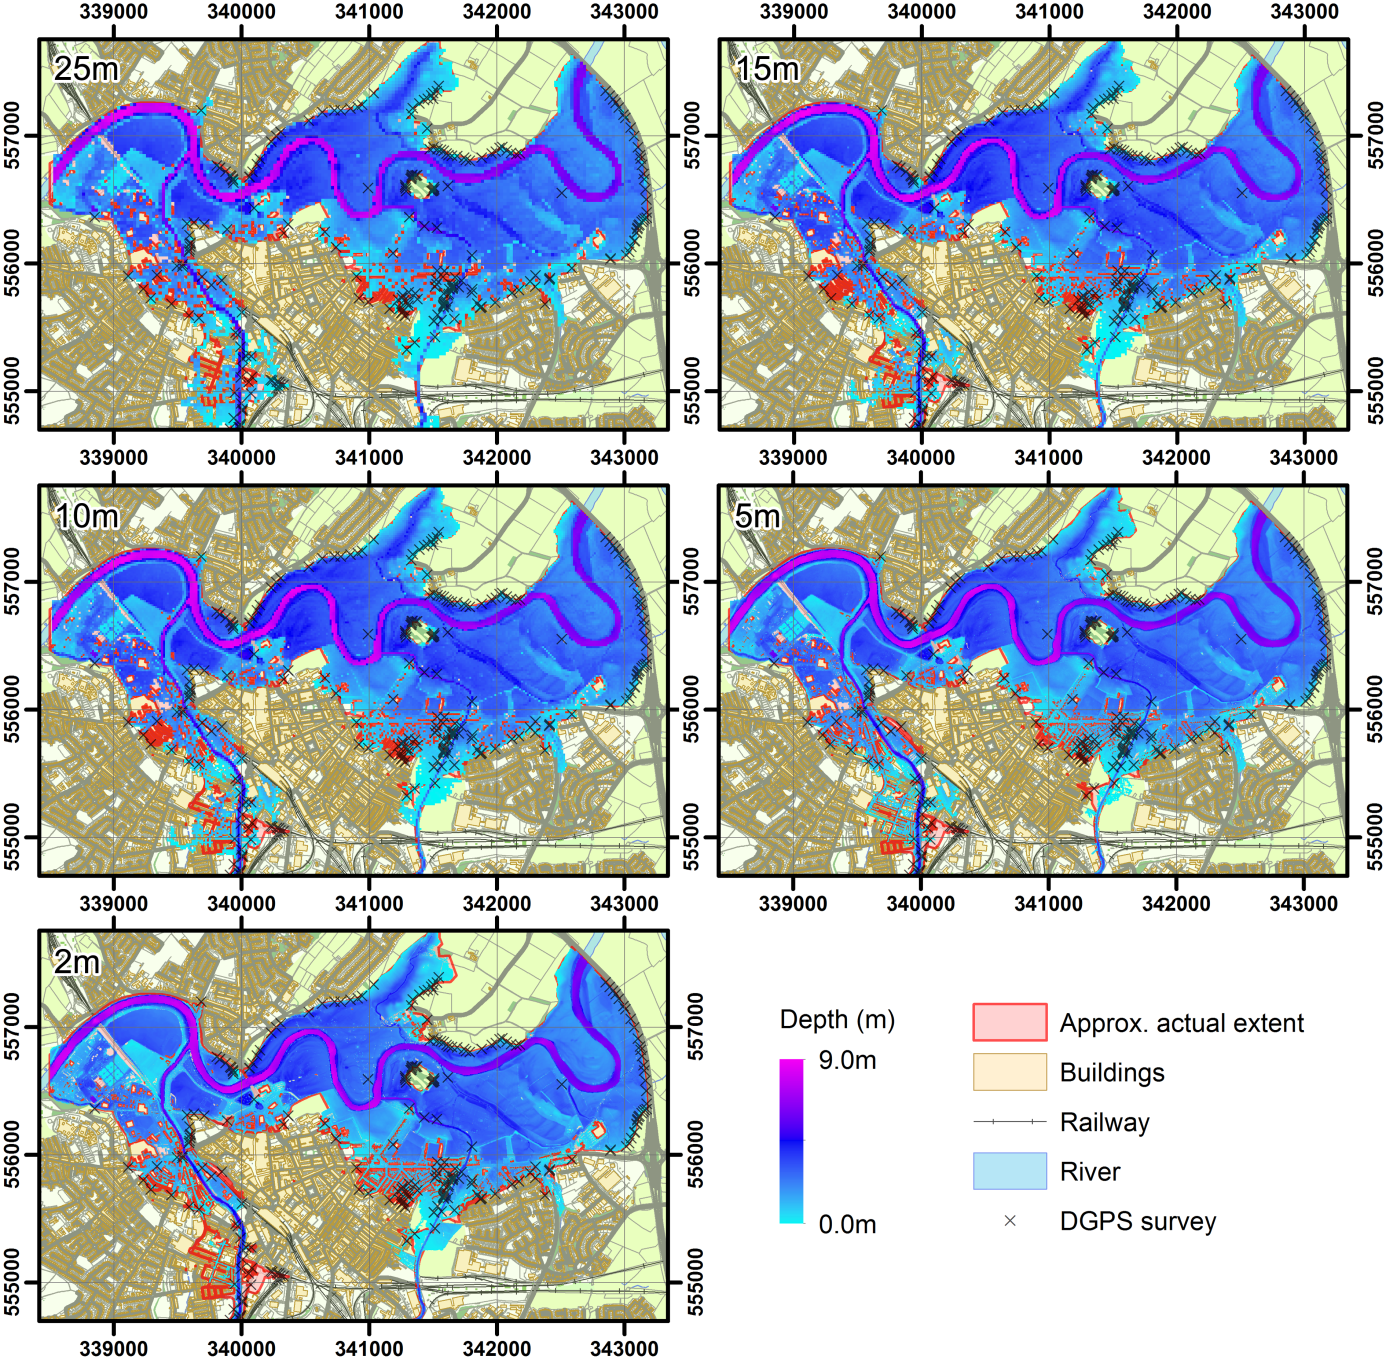
\includegraphics[width=1.0\textwidth]{carlisle-figures/Figure5.png}
	\caption{Maximum depths for calibrated simulations at different spatial resolutions.}
	\label{MaxDepths}
\end{figure*}
\begin{figure*}[tpb]
	\centering
	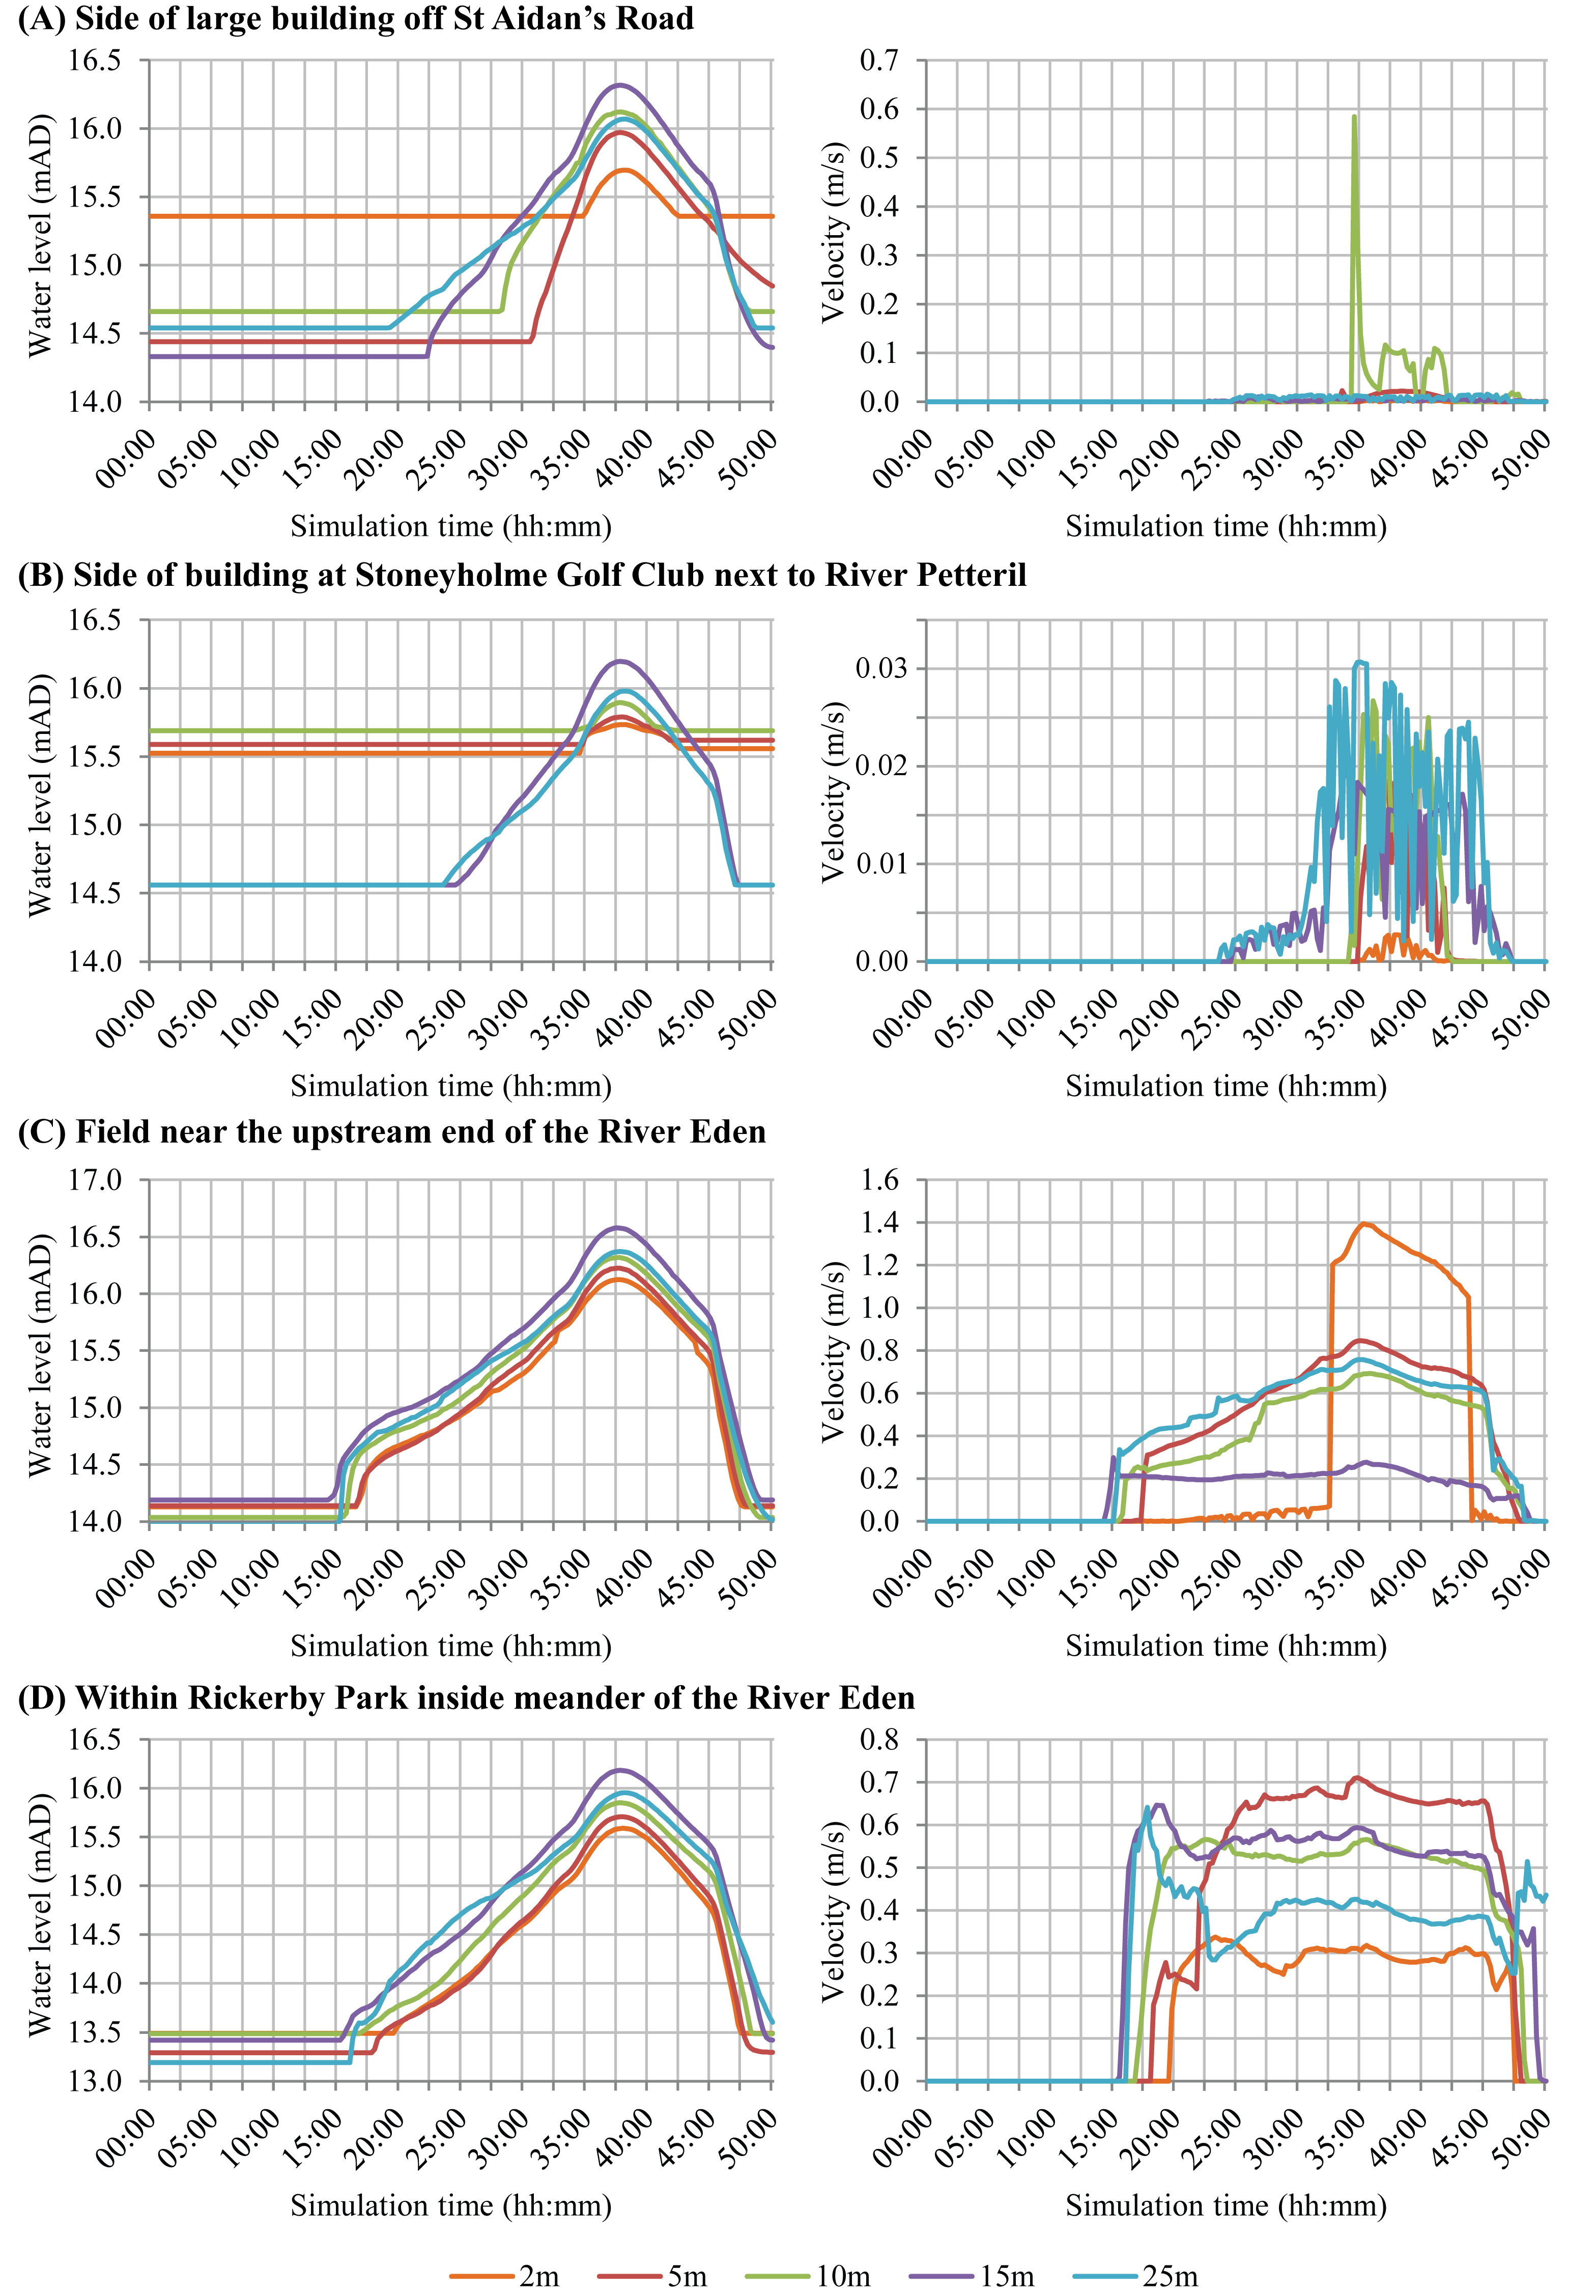
\includegraphics[width=0.93\textwidth]{carlisle-figures/Figure6.png}
	\caption{Water level and velocity plots with respect to simulation time for the four sample points identified in Figure \ref{CarlisleMap}, with fixed Manning's n of 0.04.}
	\label{TimeseriesPlots}
\end{figure*}

The value of \(C\) in equation \eqref{CFL} is taken to be 0.5 for all simulations of Carlisle, to be consistent, and accepting that some numerical diffusion may occur, but the errors present in the input datasets are likely far more significant. It is emphasised that model stability should be ensured for values up to 1.0 in idealised linear cases (as used for stability analysis), and the value selected is purely based on prior experience and analytical test cases with shocks and discontinuities \citep{Liang2009c}. Simulations were run at 5 different spatial resolutions: 2m, 5m, 10m, 15m and 25m. A downstream depth condition is imposed on the River Eden at the western edge of the domain, extrapolated from the nearby Sheepmount gauging station and thus negating its value as a further validation control. The performance of each simulation is evaluated with respect to the RMSE for the DGPS survey points, which are compared against the simulated water level for the nearest inundated cell by straight-line distance. A fit statistic \(F\) is assessed against the extent, 

\begin{equation}
	\label{FitStatistic}
	F (\%) = \frac{A - B}{A + B + C} \times 100,
\end{equation}

where \(A\) is the number of correctly predicted as inundated cells, \(B\) the erroneously predicted as inundated cells, and \(C\) the erroneously predicted as dry cells \citep[as in][]{Horritt2010}. It should be noted that this metric, although well-established, exhibits a slight preference among erroneous cells for under- rather than over-estimation, which could penalise coarse resolution simulations where terrain averaging has removed obstructions from the floodplain.

Floodplain and channel Manning's \(n\) were independently varied between the ranges of 0.02 -- 0.06 and 0.02-- 0.08 respectively at 0.01 intervals, requiring 35 simulations per resolution and 175 in total. Observations during and after the flood suggest that levels on the River Caldew upstream of a disused railway bridge were increased at least in part by debris trapped under a bridge, and that the gas works area initially flooded as a result of wall collapse \citep{EnvironmentAgency2006a,Fewtrell2011a}, which is not considered within the model. Accordingly the bias is not considered a good measure of model performance; RMSE and F are the two metrics considered to be most appropriate. A non-stationary response to calibration is found for different resolutions. Calibration of Manning's \(n\) is based on selecting the parameter pair giving the lowest RMSE against the DGPS points. This is the only uncertainty considered herein, however the hydrograph inputs used are the result of retrospective analysis of the event commissioned by the Environment Agency; a reasonable level of accuracy is hence assumed for the timeseries inputs. Selected river channel Manning's \(n\) were 0.060, 0.045, 0.020, 0.020, and 0.075 for resolutions 2m, 5m, 10m, 15m and 25m respectively. Floodplain values were 0.040, 0.050, 0.050, 0.020, and 0.020 in the same order. Maximum depths for the calibrated simulations are shown in Figure \ref{MaxDepths}, where it can clearly be seen that similar extents are attainable for all of the spatial resolutions considered herein. 

Timeseries plots of water levels and velocities at each resolution for the sample points shown on the map in Figure \ref{CarlisleMap} are displayed in Figure \ref{TimeseriesPlots}, for a uniform Manning coefficient of 0.04 for the domain including the channel. Where the water level is flat at the start of a simulation, this indicates the bed elevation of the cell which is hence dry. Velocity results vary significantly between different resolutions, however no data exist to validate velocities. Low velocities would typically be expected at point A, which is far from the watercourses and within a residential area with obstructions. Close to the River Petteril at point B, there is clear evidence that velocities vary greatly at coarse resolutions, not unexpected given that the river is less than 5m wide at this point; crucially however the time of inundation at this point is incorrectly predicted at 15m and 25m resolutions.  At point C the levels are in broad agreement across all resolutions, however a clear jump in velocities is observed at 2m resolution, which is a result of flow eventually overtopping a wall in this location only represented in high-resolution data. Levels are also in agreement at point D, however velocities vary across a range with no clear trend against grid resolutions. The 2m grid resolution consistently produces the lowest floodplain velocities, except in the case of point C as described.

\begin{figure*}[tpb]
	\centering
	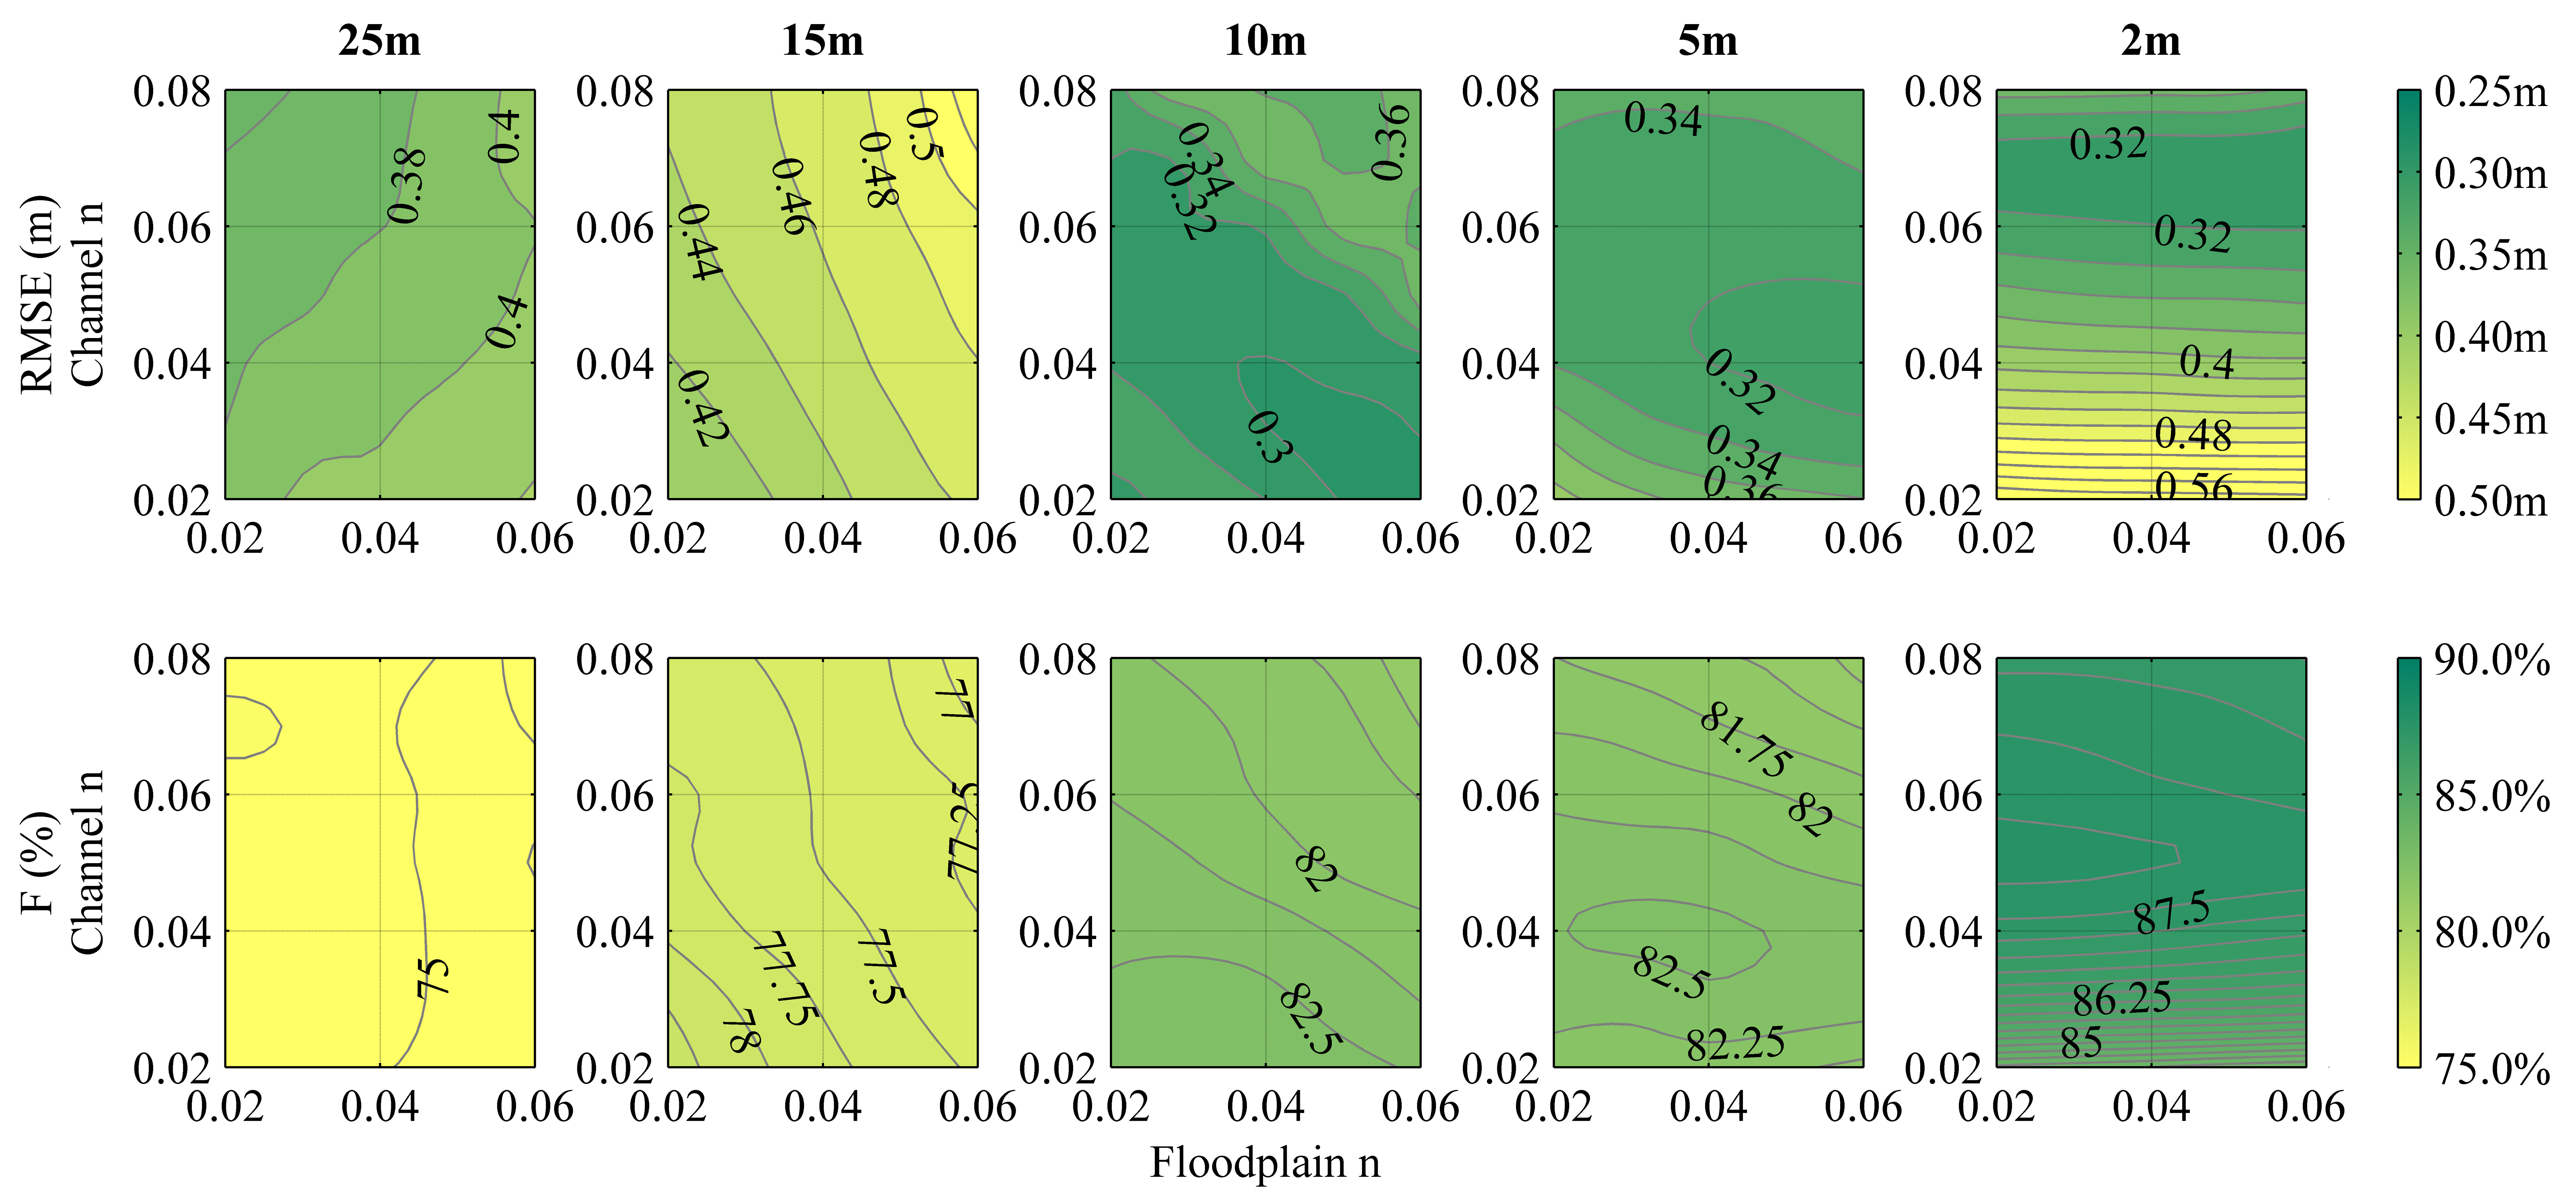
\includegraphics[width=1.0\textwidth]{carlisle-figures/Figure7.png}
	\caption{Parametric calibration for variations of Manning's n within the channel and floodplain.}
	\label{Calibration}
\end{figure*}

Further exploration of sensitivity to Manning coefficients yields interesting results. Contour plots for the biparametric calibration with the key performance metrics are shown in Figure \ref{Calibration}. Almost all of the simulations give an RMSE less than the estimated error in the DGPS measurements. At coarse resolutions optimum performance with respect to RMSE and F are not coincident. There is no consistent trend in the pattern of the optimal zones, as the resulting topography after interpolation can vary greatly at coarse resolutions owing to the size and positioning of buildings. For an increasingly fine grid, clear optimal zones emerge at 10m and 5m resolution, and by 2m only an optimal channel coefficient can justifiably be identified. For clarity at coarse resolutions no optimal zones could be found outside the calibration limits. Moreover the sensitivity changes in nature; higher resolutions show a decreasing sensitivity to the floodplain Manning's \(n\) and increased sensitivity for the channel. At 2m resolution sensitivity for the floodplain is so low that floodplain calibration barely influences the results and channel flows become the dominant factor, as confirmed by the lower velocities on the floodplain shown in Figure \ref{TimeseriesPlots} except at point C where a wall is eventually over-topped. This is not unexpected, velocities should be low for a fluvial inundation of this type, and given the meandering channel a high spatial resolution allows variations in flow characteristics within cross-sections to be properly considered.

\begin{figure*}[bp]
	\centering
	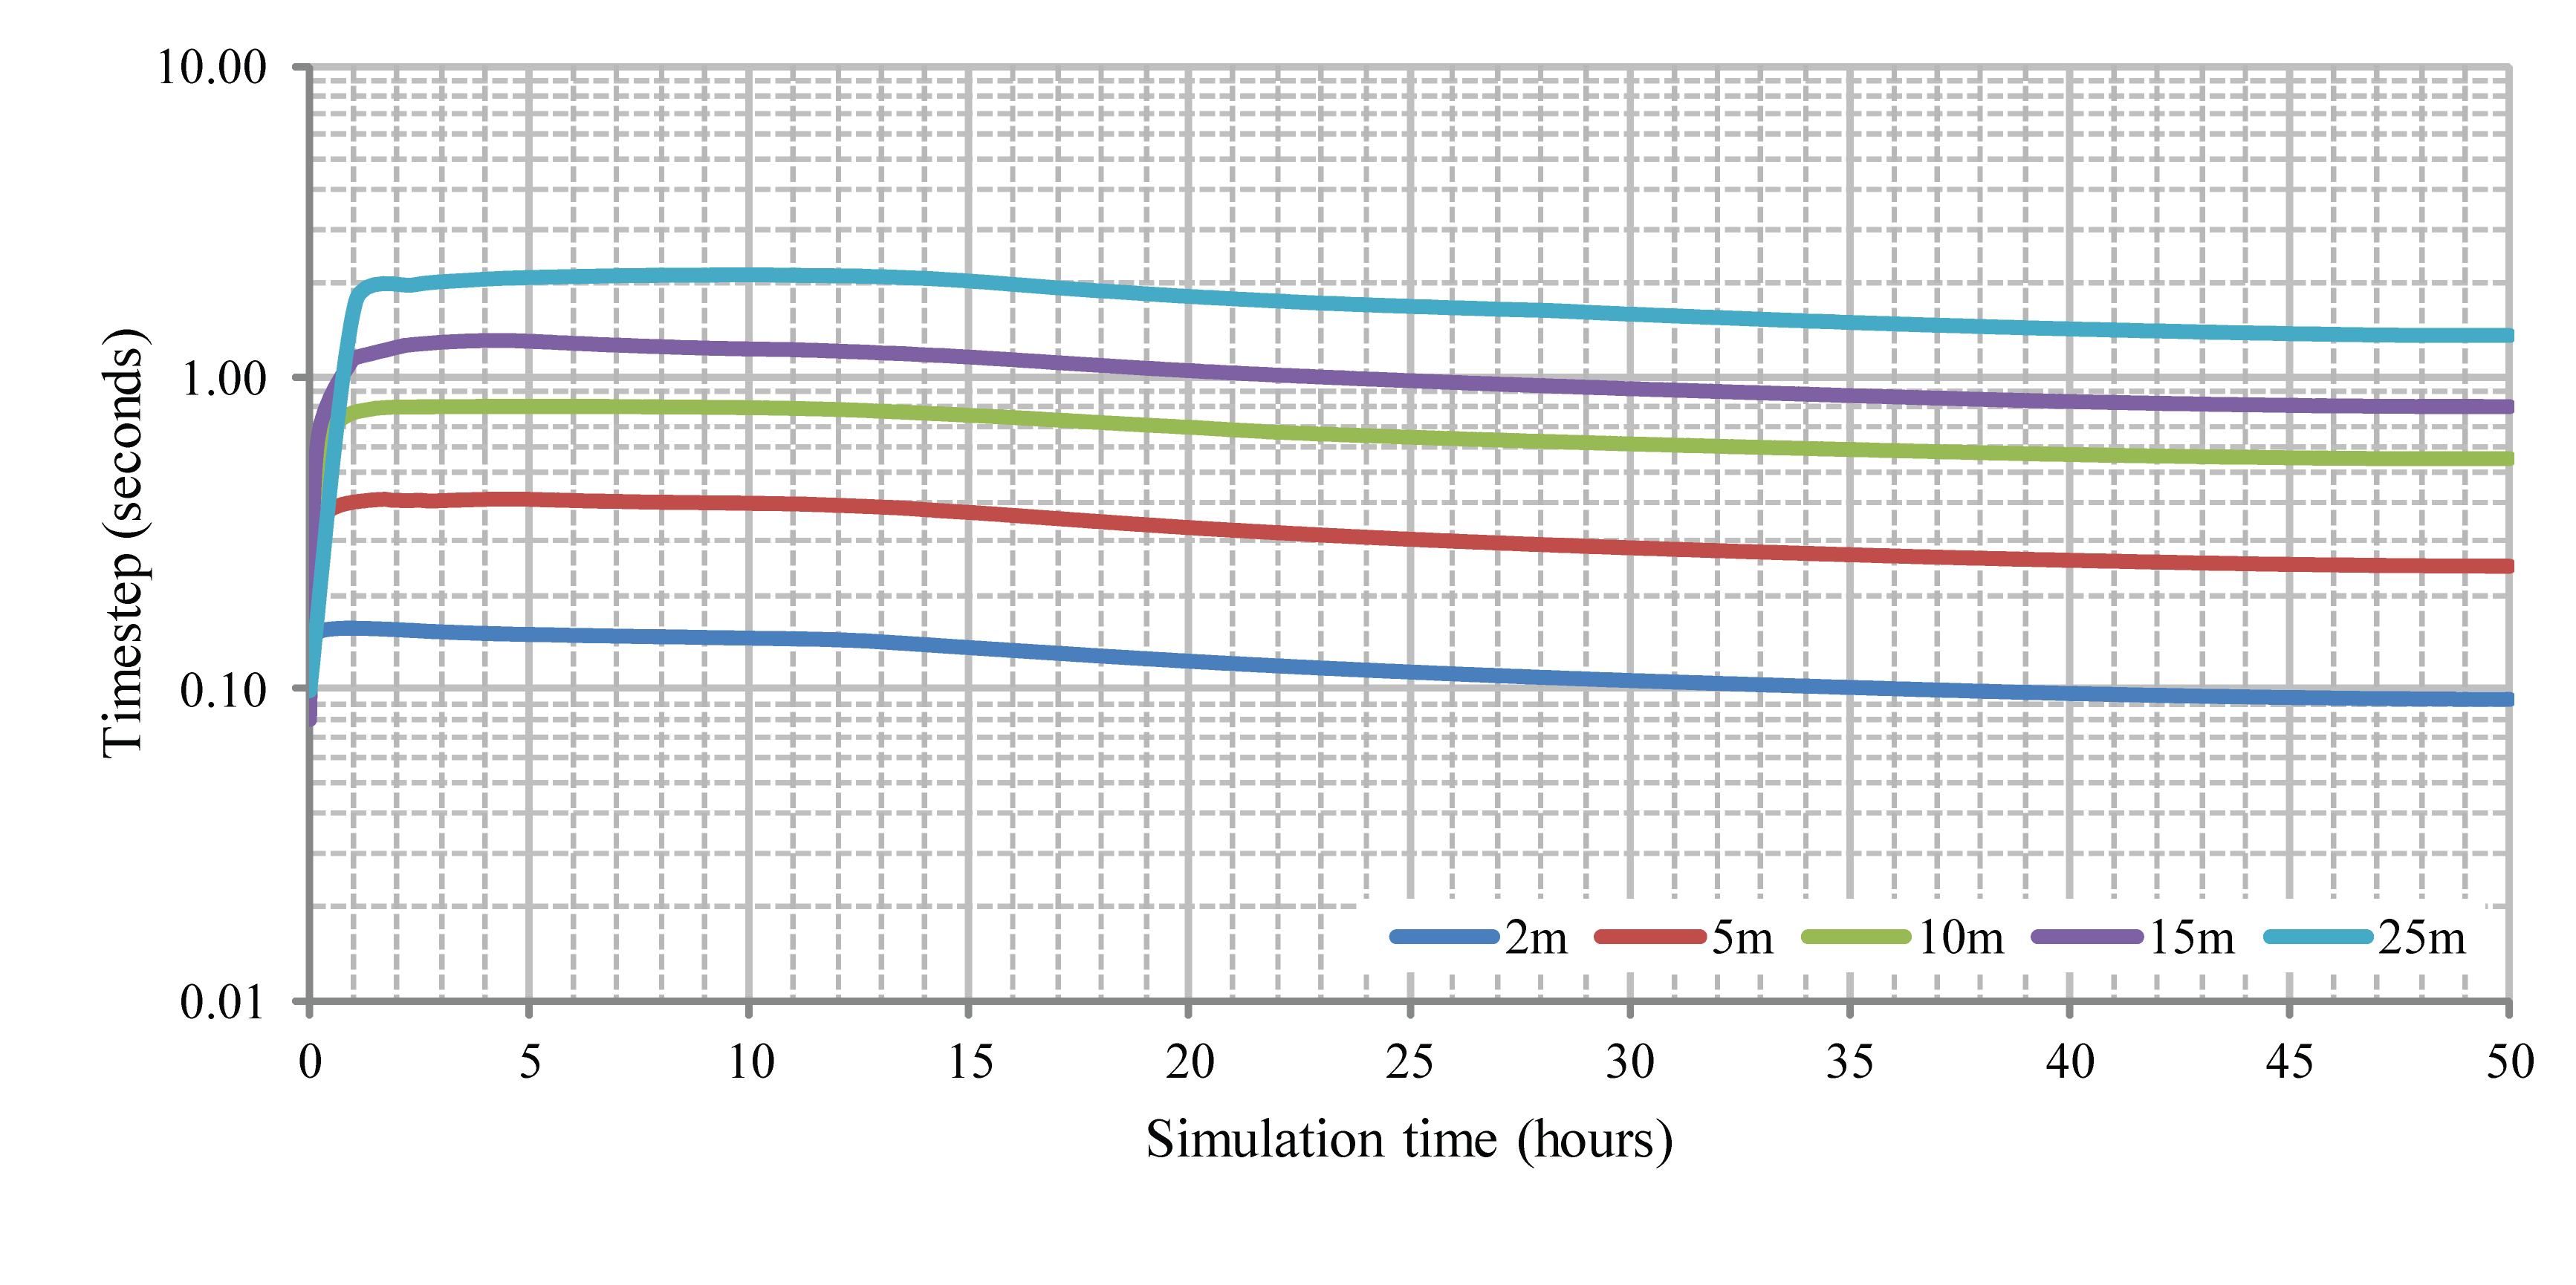
\includegraphics[width=1.0\textwidth]{carlisle-figures/Figure8.png}
	\caption{Model timesteps used throughout the 64-bit Carlisle simulations at different resolutions.}
	\label{Timesteps}
\end{figure*}

Closer examination of velocities at different intervals in the simulation shows that at coarse resolutions the flow is often circumventing the main channel due to the Cartesian grid and winding channel. Flow therefore enters the floodplain (especially in the meanders in the centre of Figure \ref{CarlisleMap} around point D) at a higher velocity, and the sensitivity to Manning's \(n\) is accordingly higher in these areas. If the low floodplain sensitivity were to hold more generally in the context of other flood events, there is clear potential for high-resolution hydrodynamic modelling with the full shallow water equations to improve accuracy in the simulation of hypothetical events, or statistically-derived scenarios. The combination of high grid resolutions and velocities in the main channel affect the timesteps shown in Figure \ref{Timesteps}, which can be as small as 0.093 seconds for the 2m simulation.

The reality however, is this event occurred close to the transitional zone of the River Eden, where slopes are minimal and the floodplain is relatively flat. Defence overtopping creates low velocities in such environments, where as water flows over the steep banks of the defences themselves, criticality is induced, and energy is lost soon after. It is essential therefore, to also consider sensitivity within the context of high flow velocities across the floodplain, such as in a catastrophic failure of the defences.

\subsection{Computational performance}

\begin{table*}[tpb]
\small
\centering
\caption{Simulation run-times for different devices, spatial resolutions and numerical precision (hh:mm:ss)}
\label{PerformanceResults}
\makebox[\linewidth]{
\begin{tabular}{llllllll}
\hline
			 		& 			& \multicolumn{2}{c}{NVIDIA Tesla M2075}			& \multicolumn{2}{c}{AMD FirePro V7800}			& \multicolumn{2}{c}{Intel Xeon E5-2609} 	\\
Resolution		 		& Cells		& 32-bit 		& 64-bit 		& 32-bit 		& 64-bit 		& 32-bit 		& 64-bit 	\\
\hline
25m					& 23,370		& 00:00:30	& 00:01:21	& 00:01:02	& 00:01:56	& 00:03:39	& 00:06:57 \\
15m					& 63,668		& 00:01:21	& 00:04:16	& 00:02:29	& 00:07:16	& 00:11:51	& 00:24:44 \\
10m					& 145,656		& 00:03:21	& 00:11:18	& 00:04:05	& 00:16:41	& 00:32:33	& 01:18:31 \\
5m					& 581,061		& 00:18:45	& 01:10:05	& 00:20:18	& 02:12:07	& 03:47:01	& 09:29:52 \\
2m					& 3,637,491	& 03:24:22	& 13:41:44	& 10:37:04	& \textit{\textgreater 40 hours}	& \textit{Not tested}	& \textit{Not tested} \\
\hline
\end{tabular}
}
\end{table*}

The time taken to simulate the first 50 hours of the event, long enough to obtain the maximum extent, is given in Table \ref{PerformanceResults}. By contrast, an NVIDIA Tesla M2075 intended for scientific computing reduces the run-time to less than 3.5 hours or 14 hours for 32- and 64-bit floating-point computation respectively. Free-surface levels and velocities are sufficiently small for this case to allow good numerical resolution and only minor differences in inundation extent when comparing 32-bit to 64-bit results. It must be emphasised that this is not true for the general case, and sensitivity analysis is always necessary before discarding 64-bit precision. It is suggested that the narrowing performance gap between NVIDIA and AMD devices with increasing resolution is a consequence of the overhead associated with launching a kernel, which becomes an increasingly small percentage of the total time. There are many factors influencing performance however. The AMD GPU is installed in a conventional workstation, and exhibits substantially reduced performance in simulations lasting more than an hour (i.e. 2m and 5m 64-bit), believed to result from hardware performance throttling because of high temperatures.

All simulations in Table \ref{PerformanceResults} were carried with using OpenCL, using all processing power and cores available for each device. Consequently even the processing time with the Intel Xeon E5-2609 CPU (quad-core with hyper-threading) represents a major reduction over many of the hydraulic modelling software packages currently used in industry, which offer no parallelisation or have been retrospectively parallelised in part using OpenMP \citep{Pender2010,Pender2013}. In such cases, where retrospective parallelisation is added, significant portions of code still execute serially and Amdahl's Law dictates that the serial portion of the program will govern the maximum reduction achievable in computation time; this limits performance increases. As expected for devices compliant with relevant IEEE standards for floating-point computation, there is no difference between the results obtained using the three different processing devices. 

As a purely indicative representation of the performance scaling achieved, the same numerical scheme programmed in FORTRAN95 and executed on a single core of the same CPU required 4.10 hours for the 10m 64-bit precision simulation. The software presented herein therefore reduces simulation times by approximately 3.1 times for the multi-core CPU and 21.8 times by using a high-end GPU for this simulation. This comparison with FORTRAN95 code should not be construed as precise; software performance on any processing device is a function of the programmer's skill, compiler used, degree of optimisation, memory access patterns, and numerous other factors. The magnitude of the speed-up with OpenCL for GPU devices is also seen to scale with increasing domain size, from 5.1 times at 25m to 8.1 times at 5m resolution, when comparing the Intel Xeon to the NVIDIA Tesla. Speed-up is dependent on a number of factors, but amongst the most significant is the proportion of dry cells; the overhead associated with launching a kernel and transferring data to registers for evaluation remains constant, but for dry cells kernels are permitted to exit early and this overhead is proportionally larger. Greater levels of speed-up relative to CPUs could be achieved for a larger domain with more immediate inundation (i.e. flash flooding), but likewise GPU computation may in fact be slower for very small domains at coarse resolutions.

\section{Hypothetical flooding in Thamesmead caused by defence failure}

The Thamesmead district of South London is located downstream of London's main flood defence, the Thames Barrier. The area is low lying but was heavily developed in the 1960s. Flood risk is posed by storm surges or a failure in the defence wall, with the area previously inundated in the North Sea Surge of 1953. A hypothetical breach in the defences is considered here, through which over 2,500,000m$^{3}$ of water enters the area with the hydrograph and entry point indicated in Figure \ref{Thamesmead_Conditions}. A 10-hour period is simulated, allowing the water to continue spreading through the computational domain.

\subsection{Model generation}

\begin{figure*}[p]
	\centering
	\begin{subfigure}[t]{0.5\textwidth}
		\centering
		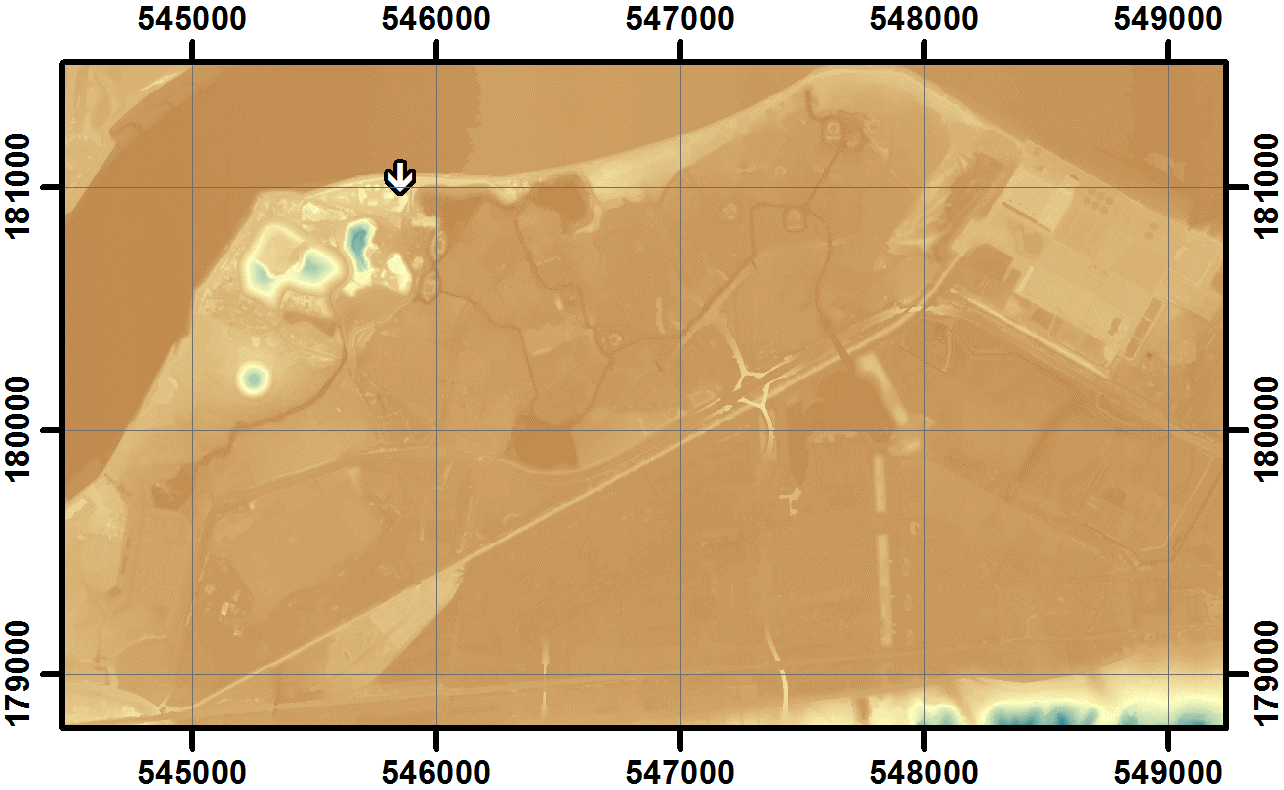
\includegraphics[width=1.0\textwidth]{heterogeneous-dev-figures/Thamesmead_DTM.png}
		\caption{Digital terrain model (DTM) and inflow location for Thamesmead}
	\end{subfigure}%
	~ 
	\begin{subfigure}[t]{0.5\textwidth}
		\centering
		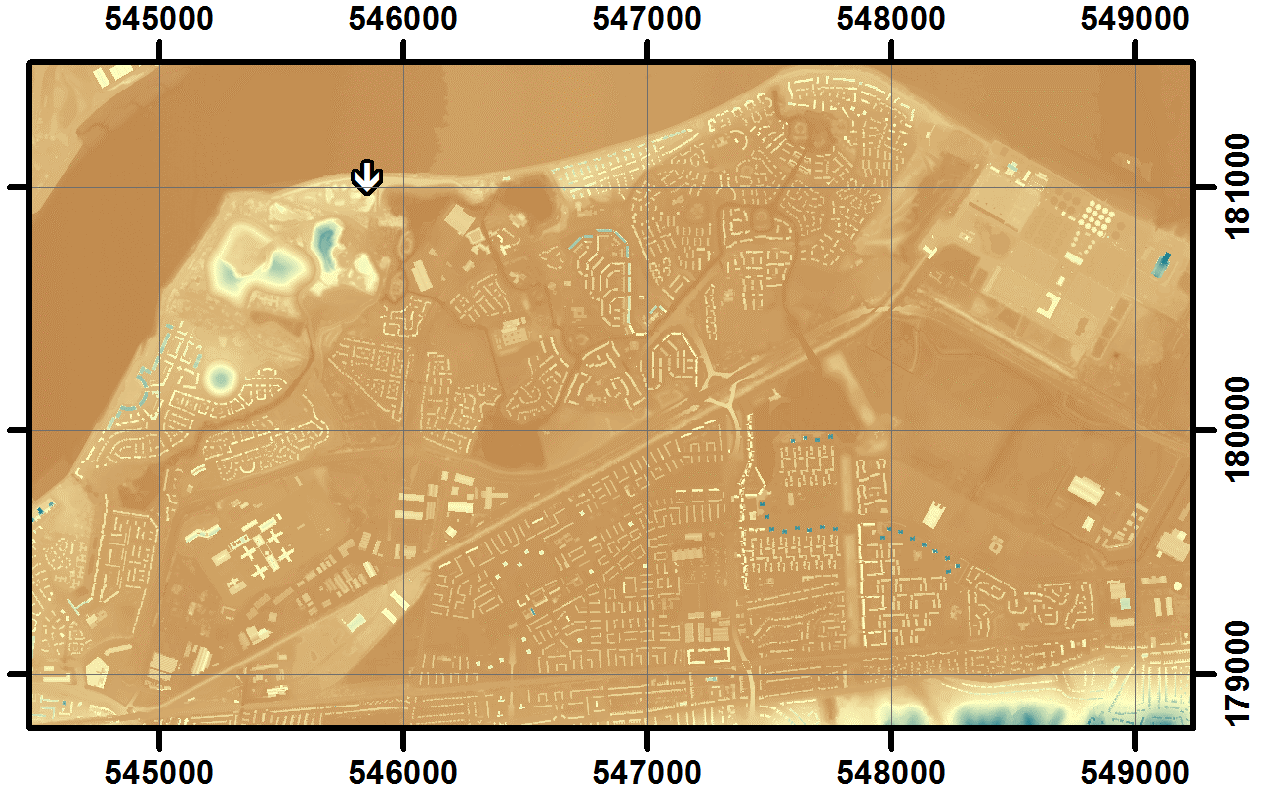
\includegraphics[width=1.0\textwidth]{heterogeneous-dev-figures/Thamesmead_DEM.png}
		\caption{Digital elevation model with buildings included (DEM) for Thamesmead.}
	\end{subfigure}
	
	\begin{subfigure}[t]{0.7\textwidth}
		\centering
		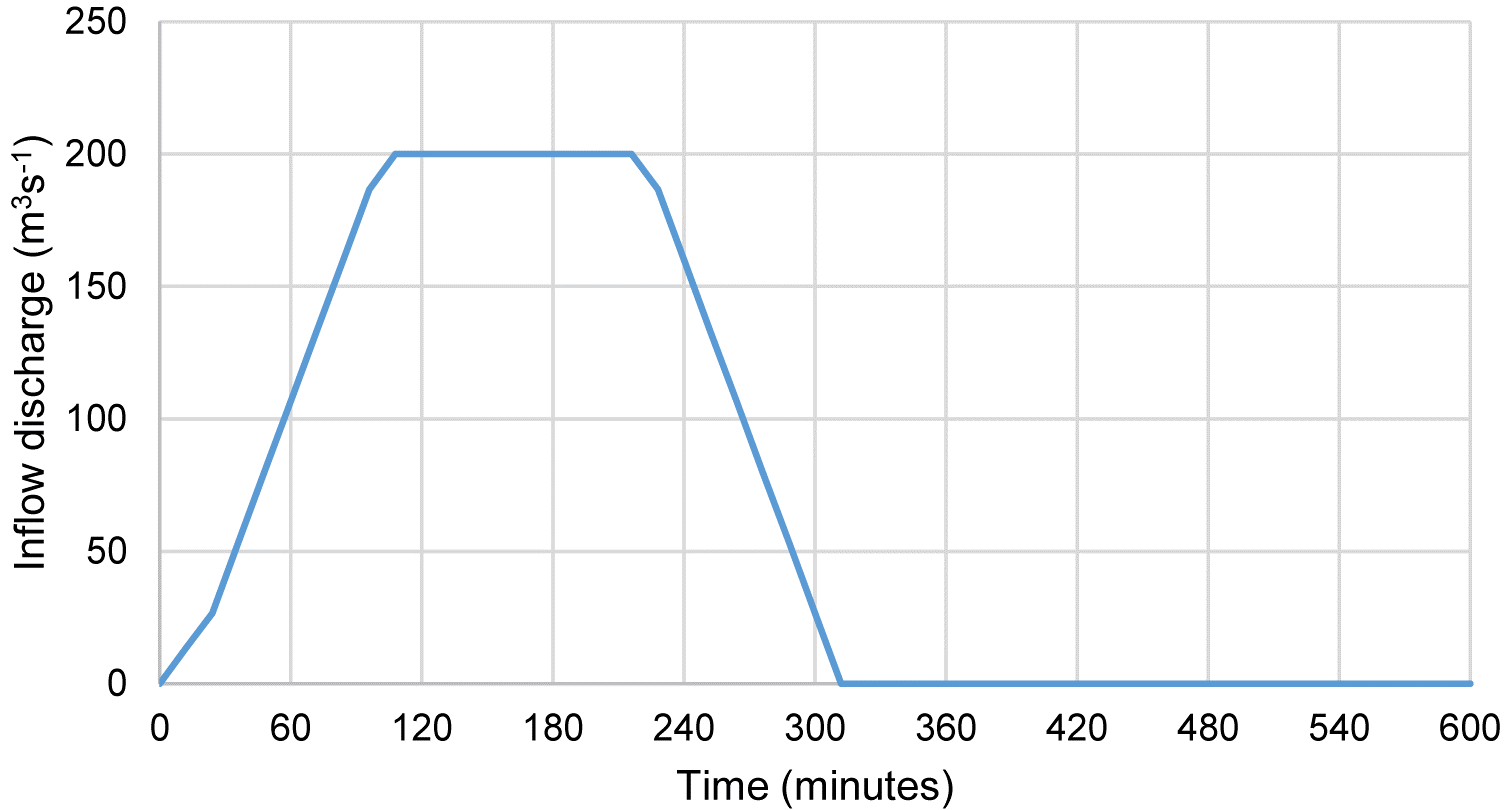
\includegraphics[width=1.0\textwidth]{heterogeneous-dev-figures/Thamesmead_Inflow.png}
		\caption{Volumetric discharge at the breach location.}
	\end{subfigure}
	\caption{Boundary conditions and topography used in Thamesmead simulations.}
	\label{Thamesmead_Conditions}
\end{figure*}
\begin{figure*}[p]
	\centering
	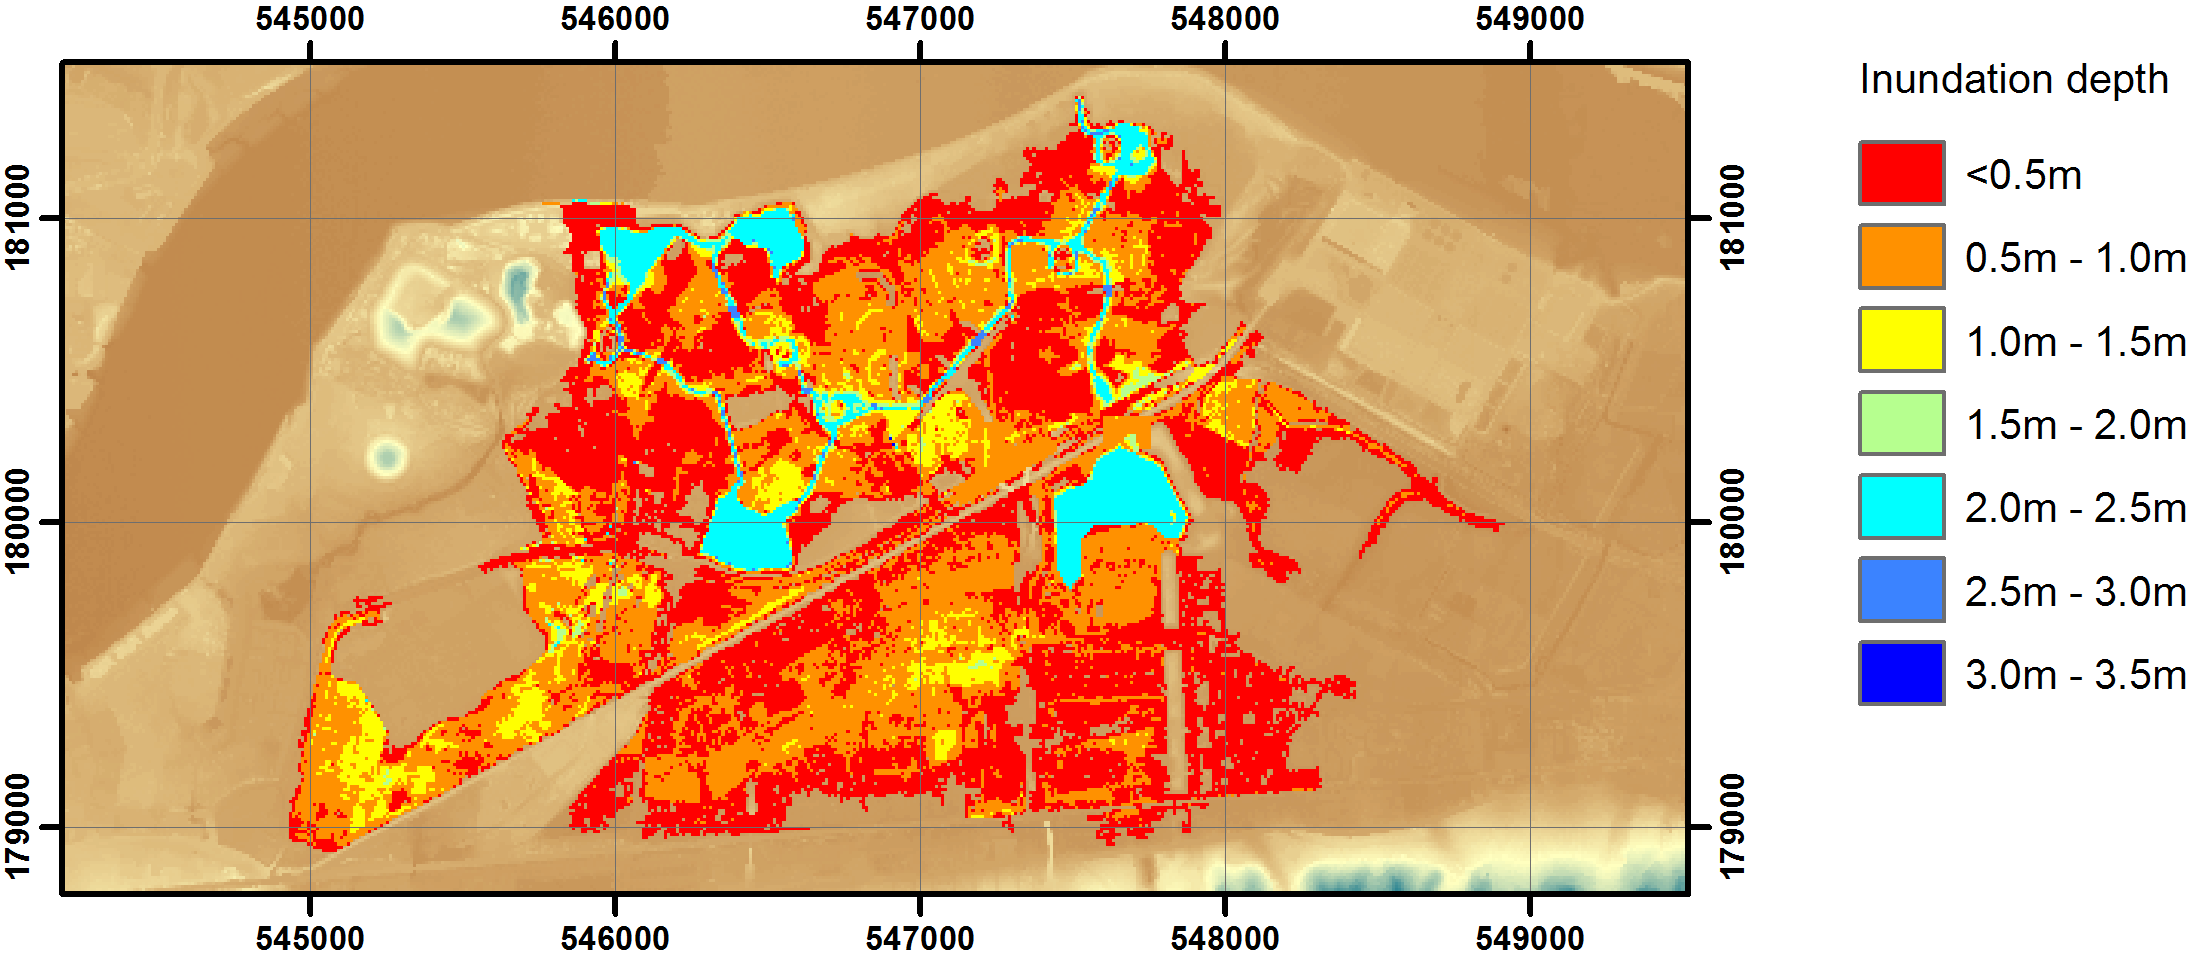
\includegraphics[width=1.0\textwidth]{heterogeneous-dev-figures/Thamesmead_10m_Comparison.png}
	\caption{Inundation results after a 10-hour period for the 10m resolution Thamesmead DTM used in \citet{Liang2010a}.}
	\label{Thamesmead_10m_Comparison}
\end{figure*}

The same hypothetical event is considered by \citet{Liang2008a}, \citet{Liang2010a}, and \citet{Vacondio2012}. These studies used a 10m resolution grid of 360,000 cells, whereby buildings and vegetation were removed from LiDAR altimetry data to create a digital terrain model (DTM). First, the simulation previously explored in literature with a 10m DTM is reproduced, in order to further validate the model. The inundation results are presented in Figure \ref{Thamesmead_10m_Comparison}, where only minimal disagreement can be identified against the results in \citet{Liang2010a}, which is effectively the same numerical scheme. This stems from differences in treatment of inflow boundary conditions for the new software, for which \citet{Liang2010a} applies imposes these on fluxes across cell boundaries, while the new software applies boundary conditions at the cell level.

The software presented herein allows us to go further. Updated datasets were created using a 2007 survey, and the resulting DTM and elevation model with buildings included (DEM) are shown in Figure \ref{Thamesmead_Conditions} at 2m resolution with 9,013,004 cells. As previously, a uniform Manning coefficient of 0.035 is applied across the domain. Cells within and north of the River Thames are excluded from computation. Transmissive boundary conditions are imposed at the domain edges. The final volume error is \textless0.1\% of the inflow volume. It can clearly be seen that a lesser flood extent is found with the new DTM in Figure \ref{Thamesmead_Inundation} for the same resolution. The updated terrain model depicts a deeper network of canals and lakes, offering increased storage.

Simulations were undertaken using both 32-bit and 64-bit floating-point arithmetic. Results presented are for 64-bit unless otherwise indicated. Whilst the average error in depth introduced by 32-bit arithmetic is small, the localised errors are in some cases unacceptably large. Errors were more pronounced at 10m resolution with the DEM; the average error exceeded 0.1m and the largest error was 0.98m. By contrast the average errors for all simulations at 5m and 2m resolution were \textless 0.01m. The magnitude of these errors is in part a function of the numerical scheme employed, where herein the free-surface level $\eta$ is used to represent cell states, to maintain depth positivity, while some numerical schemes achieve this through alternate means, potentially allowing greater precision when storing low depths. As an example, a depth of $0.001234$ is stored under IEEE 754 using 1 bit for sign, 8 bits for an exponent, and 23 bits for the integerial 'fraction' raised to the exponent to produce the actual value, i.e. $2^{-10} \times 1.2636159 \approx 0.001233999$; larger values such as the free-surface level limit the exponent, hence the fraction bits provide a lower numerical precision. Nonetheless, it would not be surprising if coarse resolutions are more sensitive to numerical resolution given the larger volume affected by the same change in depth. Further research is required.

\subsection{Effect of grid resolution and parameterisation}

\begin{figure*}[p]
	\centering
	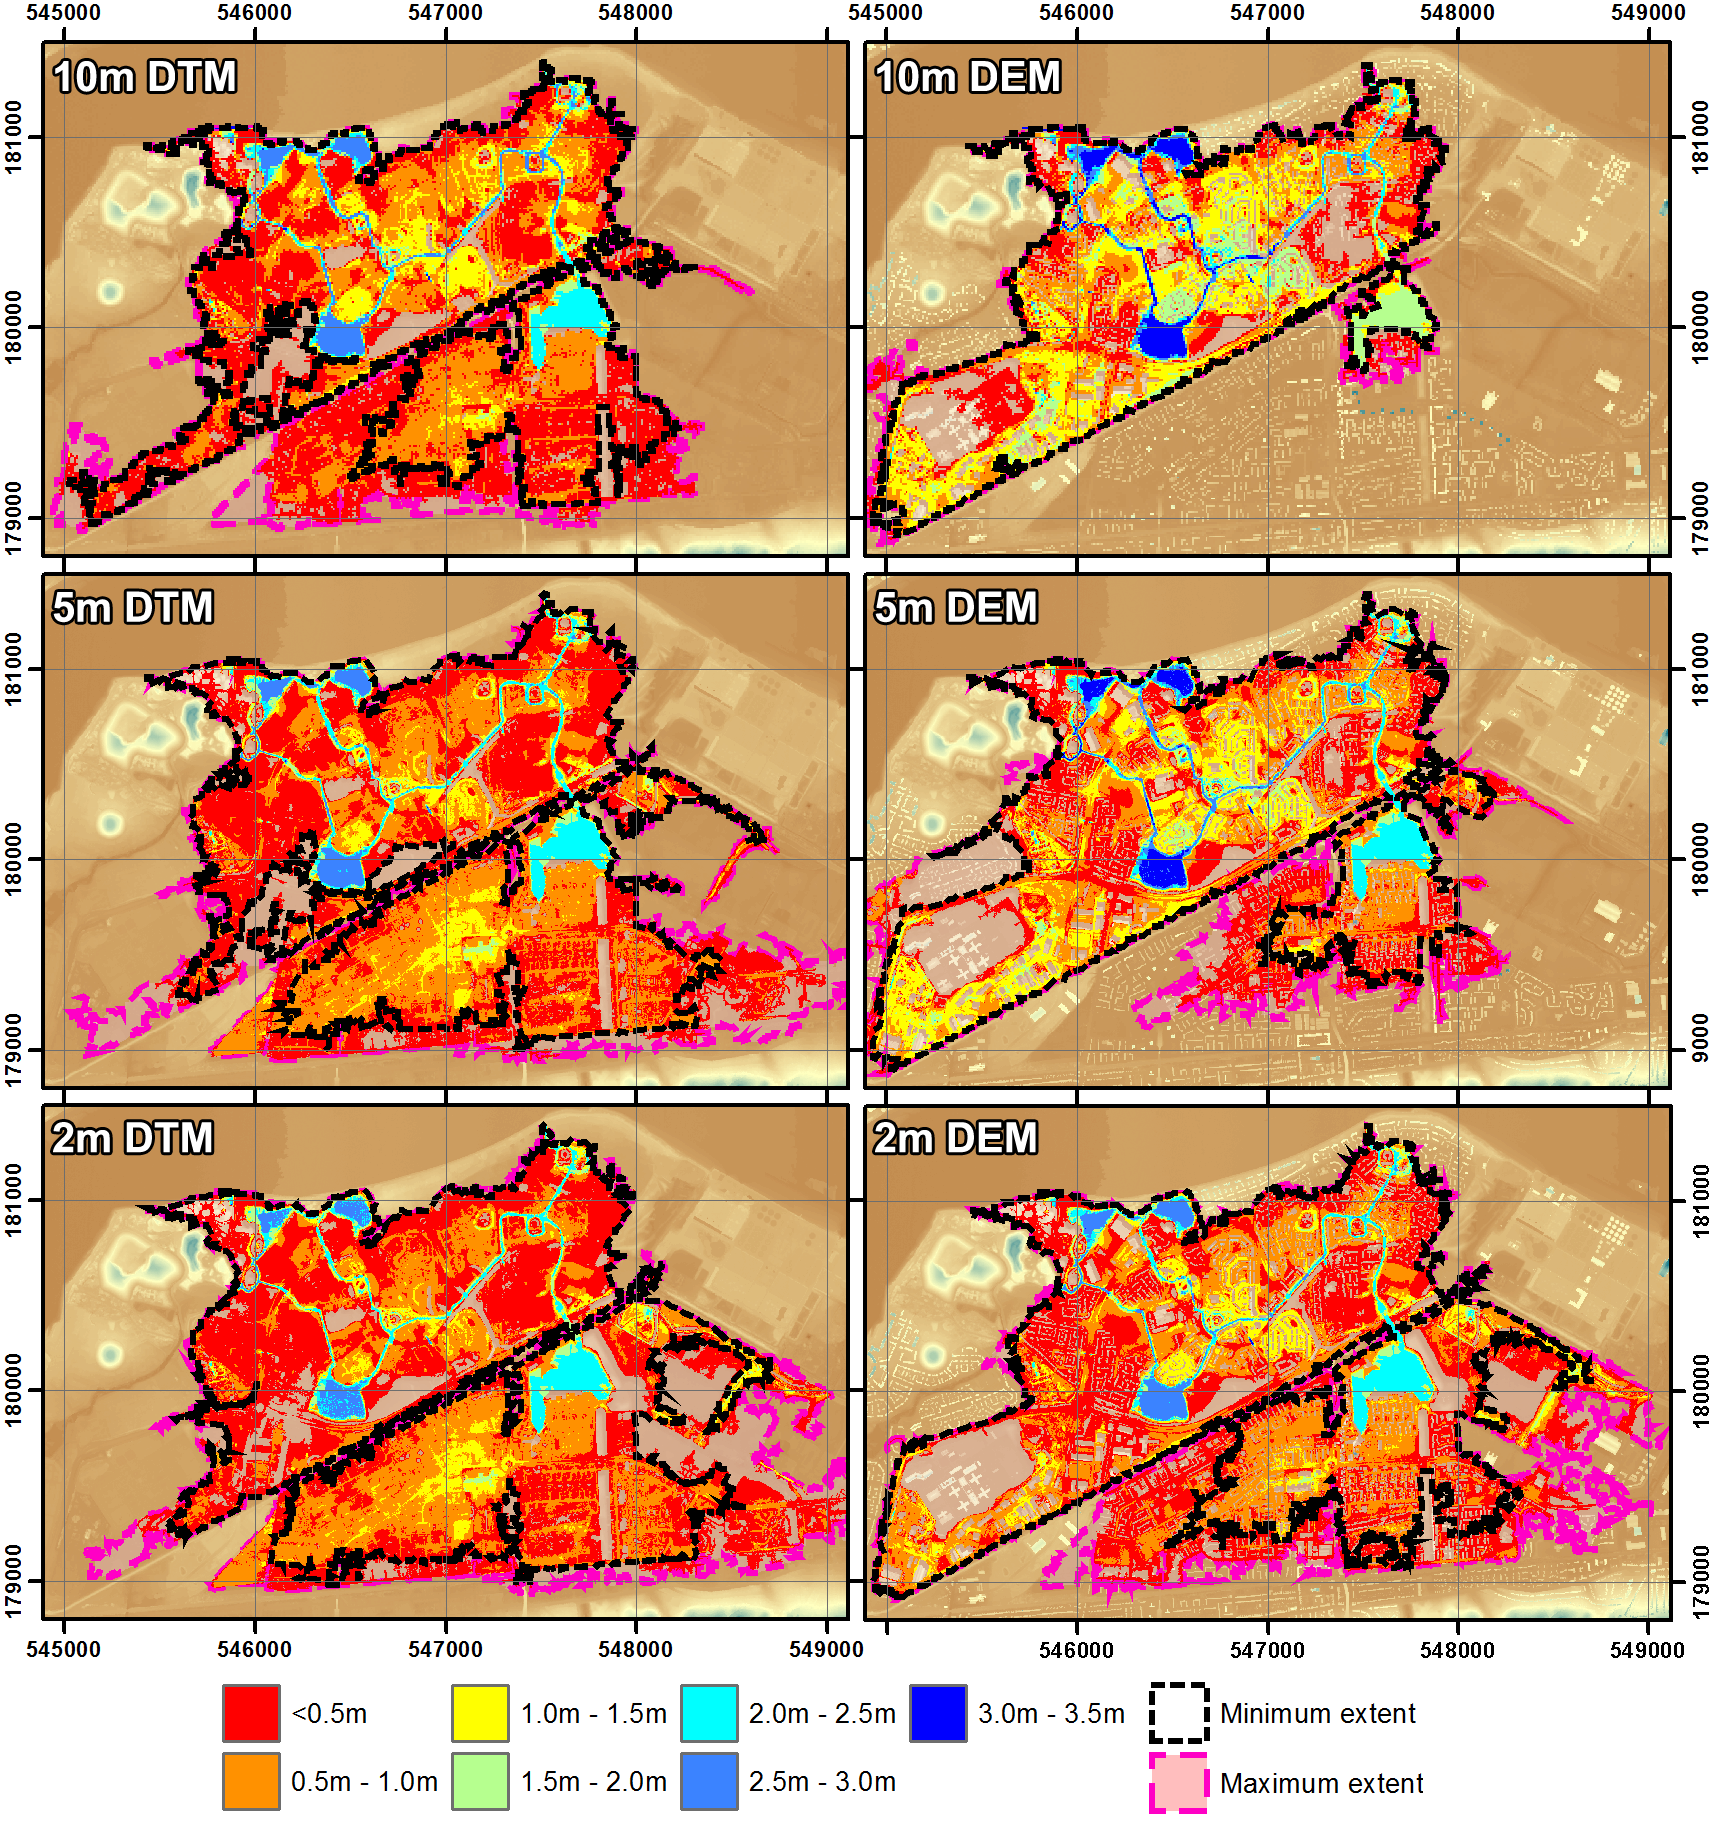
\includegraphics[width=1.0\textwidth]{heterogeneous-dev-figures/Thamesmead_AllDepths.png}
	\caption{Inundation results after a 10-hour period using DEM and DTM at different spatial resolutions, and the minimum and maximum inundation extents with Manning values from 0.01 to 0.09.}
	\label{Thamesmead_Inundation}
\end{figure*}
\begin{figure*}[p]
	\centering
	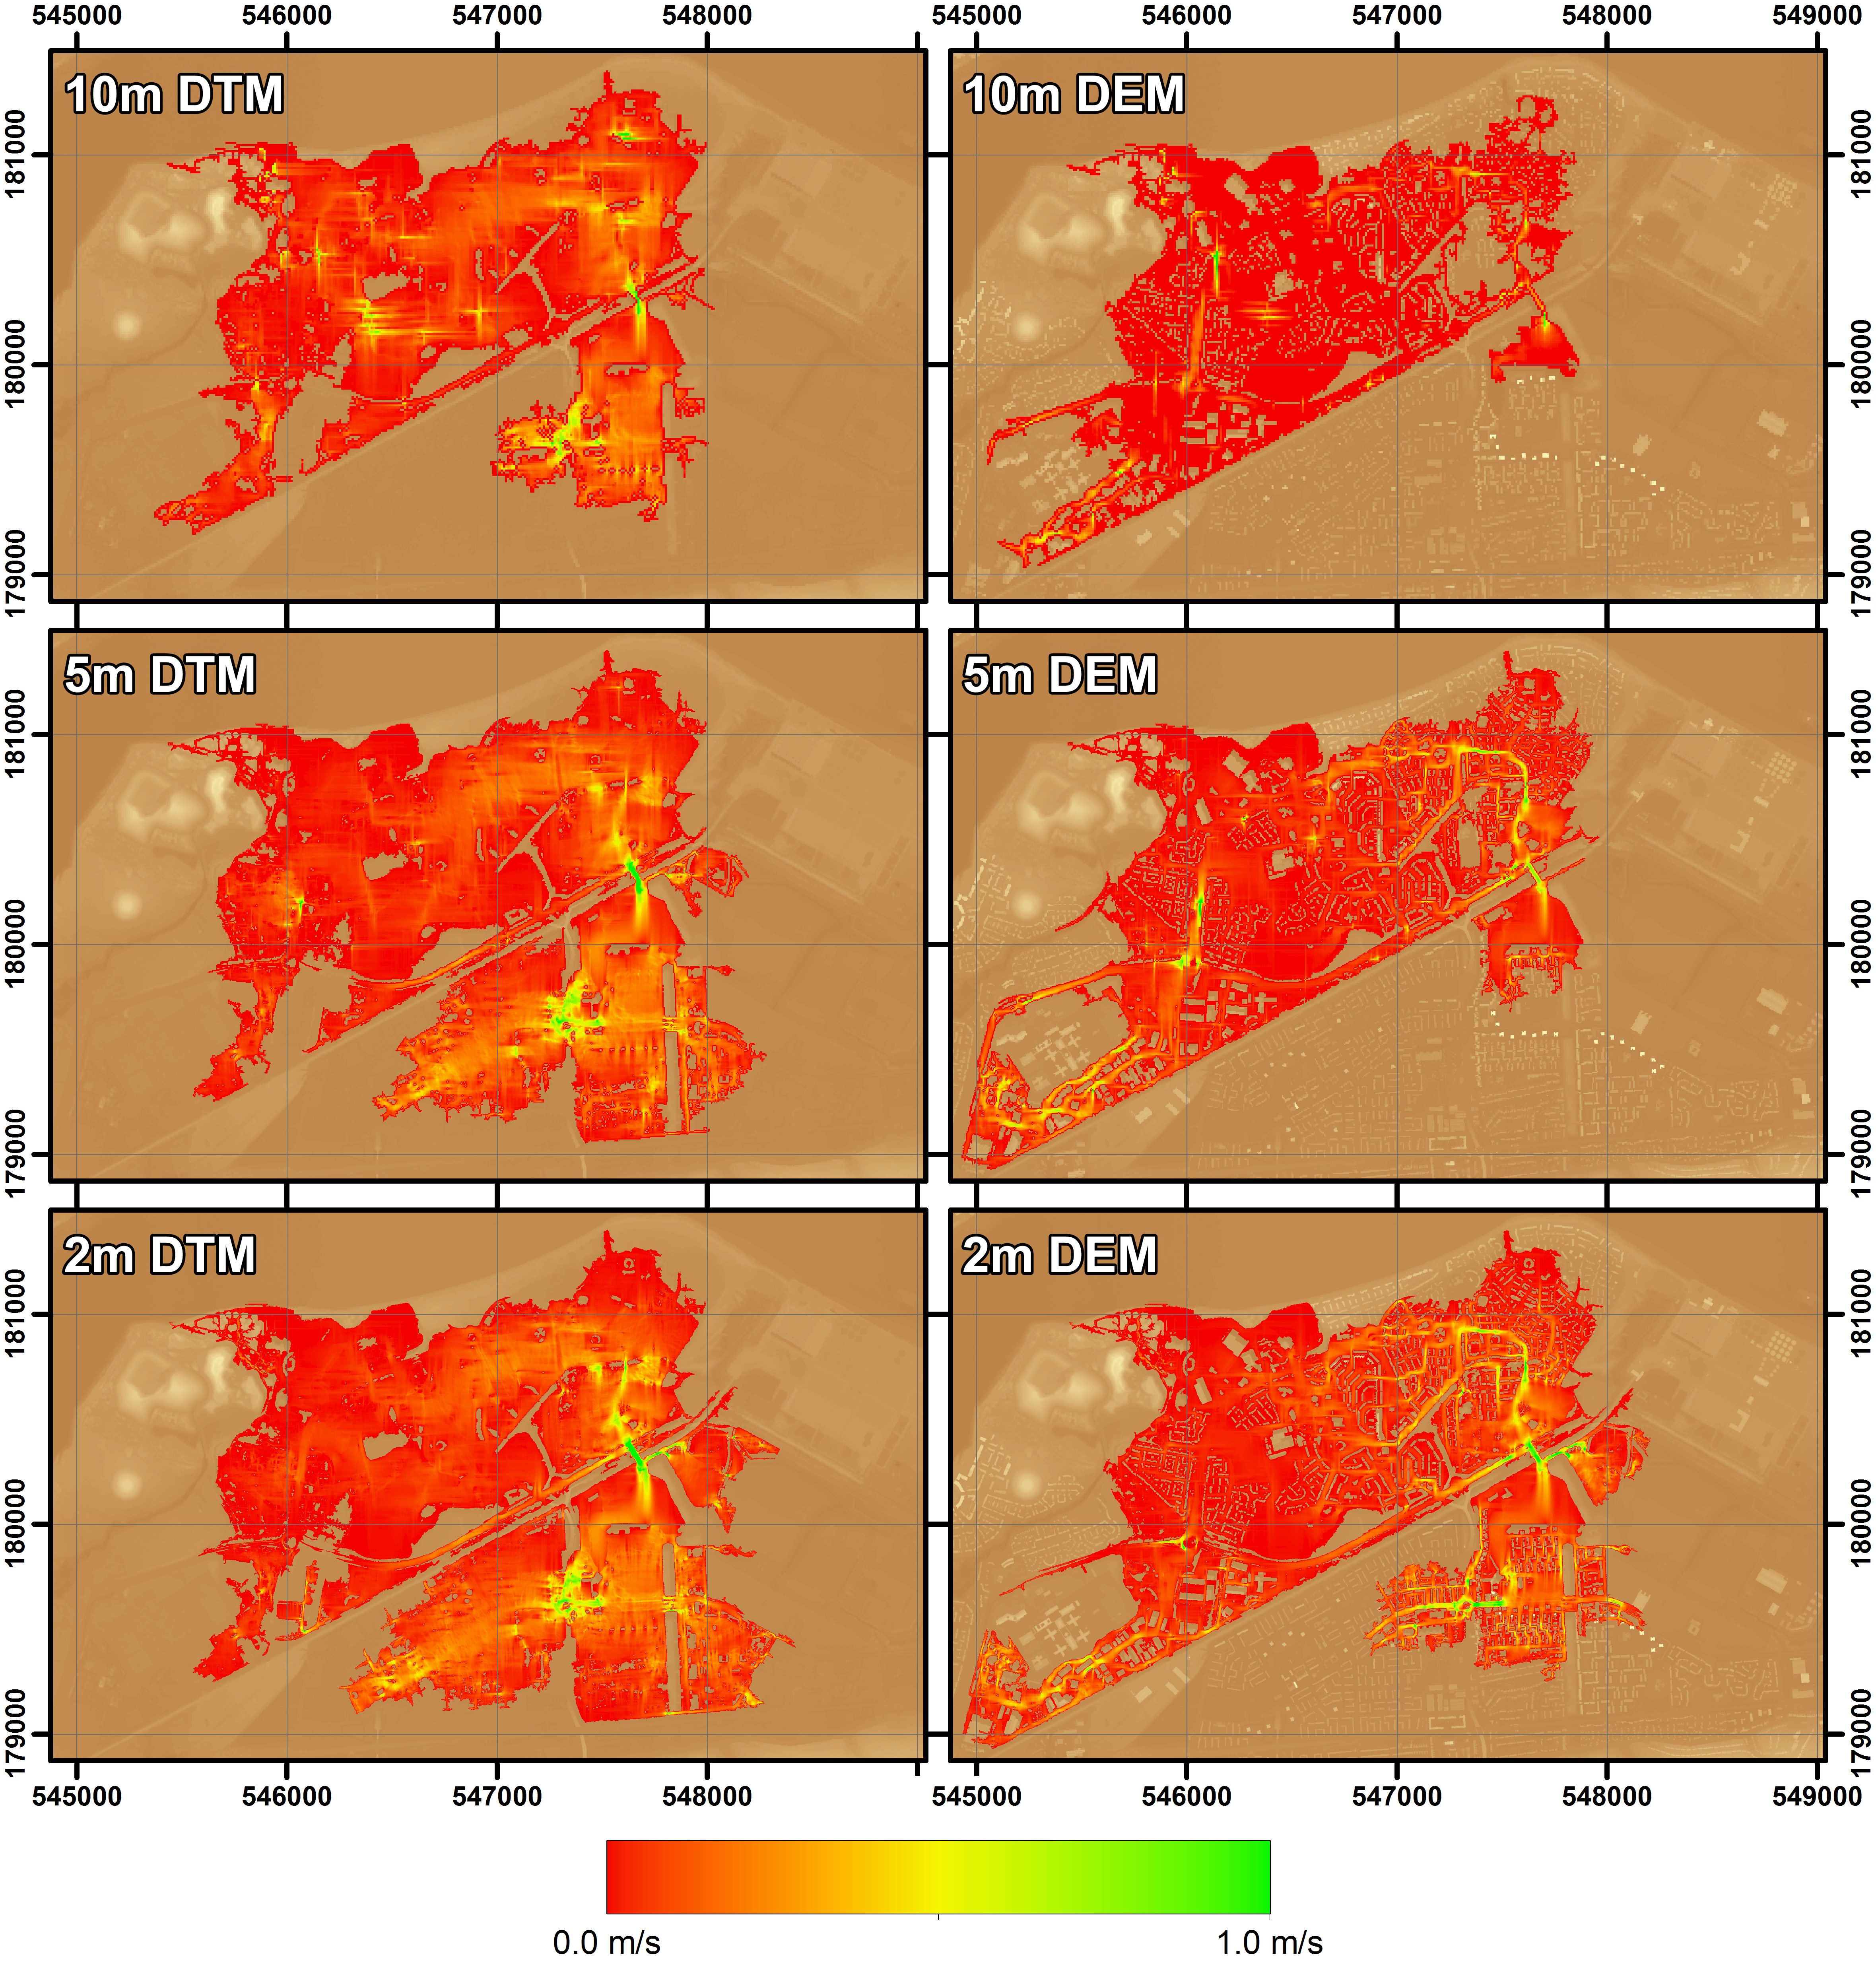
\includegraphics[width=1.0\textwidth]{heterogeneous-dev-figures/Thamesmead_AllVelocities.png}
	\caption{Magnitude of velocities at 6 hours using DEM and DTM at different spatial resolutions. }
	\label{Thamesmead_Velocities}
\end{figure*}

The final extent and inundation depth for the three resolutions and two elevation models employed are shown in Figure \ref{Thamesmead_Inundation}. The building layout is unusual in Thamesmead, with numerous connected networks of buildings. Small tunnels and alleyways allow for pedestrian access, and the elevation models have been adjusted to ensure these are present as a flow pathway. These passages are small however, hence the buildings can be expected to reflect a large volume of the flow impacting them; this is confirmed by the results obtained. Inclusion of buildings results in an increased inundation in the west of the domain. Spatial resolution also has a substantial impact on the flood extent. Figure \ref{Thamesmead_Velocities} shows the magnitude of the velocities after six hours, with the highest velocities present at the highest resolutions where narrow gaps are clearly resolved, concentrating flow to alleyways and streets. As a consequence flood progression is more rapid at higher resolutions. In this case, coarse resolutions may result in underestimation of flood extent.

Additional simulations were run for each grid resolution with different Manning's $n$ values from 0.01 to 0.09 at 0.02 increments, giving 30 simulations in total. This allows the sensitivity to parameterisation to be assessed, representing an envelope of uncertainty which in the real-world may be street furniture, vegetation, and obstructions such as vehicles. The minimum and maximum extent of flooding after 10 hours across the calibration range is shown in Figure \ref{Thamesmead_Inundation}. As expected, a lower Manning's $n$ results in a larger area of inundation by the end of the simulation. Consistent with the findings of \citet{Yu2006}, coarser grid resolutions exhibit lower sensitivity to Manning's $n$, while there is a substantial range in final extent for both the DEM and DTM at 2m resolution. This is unsurprising given the higher localised velocities at fine grid resolutions. Low sensitivity to parameterisation at coarse grid resolutions is not a justification for using these resolutions however, as the difference in inundation from coarse to fine resolution grids far exceeds the scope of influence any parameterisation might have. Consequently there is a clear need for sub-grid scale representation of topographic features, dynamically adaptive grids, or use of high-resolution grids throughout. 

The high-velocity nature of this hypothetical event contributes to the higher sensitivity, in contrast to studies exploring slow fluvial floodplain inundation by overtopping of defences rather than breach. \citet{Fewtrell2011a} demonstrate that floodplain sensitivity is significant in both a LISFLOOD and ESTRY-TUFLOW simulations of the Carlisle 2005 flood, using a 25m grid. However a more detailed representation of the in-channel flow dynamics using a high resolution grid and shock-capturing scheme throughout is shown to decrease floodplain sensitivity to have very little effect with a 2m grid for the same event by \citet{Smith2015}, and as described previously in this chapter.  Evidently, high-resolution simulations alone are insufficient for flood risk analyses in defence breach situations, requiring comprehensive exploration of inundation with different parameterisations to fully assess the potential consequences for hypothetical and statistically-derived flood events. At its most extreme, the use of coarse grids and a single Manning's $n$ in broad-scale flood risk analysis could significantly underestimate the threat, as demonstrated by the marked differences in results obtained herein.

\subsection{Computational performance}

First, performance is considered for the 10m simulation, to allow comparison with other studies of the same scenario. \citet{Liang2008a} reports a run-time on a computer of that era, in excess of 4 hours, demonstrating the scale of the improvement in a relatively short period of time, even without leveraging GPU computing. The Thamesmead simulation involves approximately four times the number of cells, when compared to the Glasgow test case presented in Chapter \ref{chapter:NumericalValidation}, however the different nature of the event means many of the cells will be dry, thus calculation may shortcut in these cases. The performance results presented in Table \ref{ThamesmeadPerformance} again show a clear performance advantage for GPUs against CPUs, as expected. The inferior GPU is again faster in both 32- and 64-bit computation, suggesting the 360,000 cells remain insufficient to mask the GPU transfer and dispatch overheads. Despite the increased cell count, some simulations are faster for Thamesmead than Glasgow, suggesting the number of inundated cells is highly influential in performance results. Accordingly, pluvial flooding is expected to be among the most computationally demanding of scenarios.

\begin{table*}[tpb]
	\newcolumntype{R}[1]{>{\RaggedLeft\arraybackslash}p{#1}}
	\small
	\centering
	\caption{Simulation run-times for Thamesmead in minutes using three different processing devices at different resolutions and DEM or DTM.}
	\label{ThamesmeadPerformance}
	\begin{tabular}{p{0.1\textwidth}p{0.1\textwidth}p{0.15\textwidth}R{0.15\textwidth}R{0.15\textwidth}R{0.15\textwidth}}
		\toprule
		\raggedright{Cell elevations} & \raggedright{Spatial resolution (m)} & \raggedright{Floating-point arithmetic resolution} & CPU Intel Xeon E5-2609 & GPU AMD FirePro V7800 & GPU NVIDIA Tesla M2075 \\
		\midrule
		DTM		& 	10	&	32-bit 	&	10.53	&	0.73	&	0.83 \\
		&		&	64-bit 	&	23.50	&	1.88	&	2.40 \\
		& 	5	&	32-bit 	&	47.20		&	2.78	&	3.25 \\
		&		&	64-bit 	&	109.12	&	10.50	&	10.33 \\
		& 	2	&	32-bit 	&	636.72	&	40.43	&	40.20 \\
		&		&	64-bit 	&	\textgreater 1,800.00 	&	154.25	&	137.88 \\
		DEM		& 	10	&	32-bit 	&	10.57	&	0.77	&	0.85 \\
		&		&	64-bit 	&	10.87	&	1.92	&	2.35 \\
		& 	5	&	32-bit 	&	50.55	&	3.03	&	3.45 \\
		&		&	64-bit 	&	118.20	&	10.68	&	10.97 \\
		& 	2	&	32-bit 	&	675.18	&	40.73	&	40.20 \\
		&		&	64-bit 	&	\textgreater 1,800.00	&	147.62	&	137.70 \\
		\bottomrule
	\end{tabular}
\end{table*}

Total simulation times for a 10 hour period in Thamesmead with different processing devices are given in Table \ref{ThamesmeadPerformance}. The software presented herein takes advantage of all four CPU cores made available to it, giving a much more realistic comparison between the achievable performance of GPU and CPU devices than comparisons against single-threaded code which may not have been optimised. Multiple orders of magnitude speed-up should not be expected when comparing against optimised code, based on vendor-quoted performance figures \citep{Brodtkorb2012,Smith2013}; examination of device peak compute power in terms of floating point operations per second (FLOPS) reaffirms that such dramatic levels of performance boost are highly unlikely. The AMD device performs well in all of the simulations, at speeds which are comparable to NVIDIA, but retailing at a much lower price. For large domains with millions of cells it is possible to reduce simulation time to a fifteenth or less of the multi-core CPU equivalent for the software presented herein.

\section{Conclusion}

This chapter has presented a real-world application of the new computational techniques, providing accurate results consistent with observations taken after the event. However, when the same methods are applied to a defence failure event, in which high velocities are encountered on the floodplain instead of only the river channel, sensitivity becomes a far greater concern. There are a number of observations and limits to consider in future simulations.

\begin{itemize}
	\item Lowering the numerical precision to 32 bits provides a substantial performance benefit in this case, where velocities are low and flooding is gradual over a long period. However, in advance of a simulation one could not definitively say that 64-bit precision would not be required; even a gradual event may have short time periods where velocities are high, or the cumulative effect of the small errors could eventually create a much greater deviation; it is the author's opinion that the performance benefits of 32-bit processing cannot be leveraged without full sensitivity analysis conducted first.
	\item Parameterisation is not transferable between different grid resolutions, as might be expected. The Manning coefficient is used to factor energy loss not fully captured elsewhere in the model, most notably that of friction, but a more refined grid resolution should capture a greater proportion of the flow characterisations from the real world, hence the correction required should decrease for gradually-progressing floods. In reality, the extent of these losses is spatially-varying, thus the Manning's $n$ should be spatially distributed; an inaccurate simplification was used here to allow exploration without excessive numbers of parameters, where only the river channel and floodplain were differentiated for Carlisle.
	\item High-velocity flood events, such as those caused by defence failure, are extremely sensitive to both the grid resolution and parameterisation. Failure to use a high-resolution mesh could seriously underestimate flood risk, especially in urban environments where the built environment provides narrow flow corridors which can exacerbate flow velocities.
	\item Marked differences are observed by using a DTM versus a DEM with buildings included, whereas the reality probably lies somewhere in between (i.e. above a threshold height, windows and airbricks would be expected to convey water through a building).
	\item External factors such as hardware throttling (where performance is artificially reduced to manage temperature or power) are difficult to quantify, as they are controlled by proprietary systems and software.
	\item Clear benefits in the refinement of the flood event are seen when using high grid resolutions which capture the topographic complexity, however the simulation run-times even with high-performance GPUs are still long.
\end{itemize}

Considering the run-time at high resolutions, and the potential need to run multiple simulations across a range of parameterisations to fully capture a range of outcomes, further performance improvements are required. Increasing the number of processing devices used is considered next.
